\documentclass[a4paper,10pt]{report}
\usepackage[utf8]{inputenc}
\usepackage{fullpage}
\usepackage{amsmath}
\usepackage{amsfonts}
\usepackage{tikz}
\usepackage{graphicx}
\usepackage{mdframed}
\usepackage{color}
\usepackage{listing}
\usepackage{wrapfig}
\usepackage[parfill]{parskip}
\usepackage{subcaption}
\usepackage{hyperref}
\usepackage[font={small}]{caption}
\usepackage{marvosym}
%-----------------------------------------------------
% Drawing packages
%-----------------------------------------------------
\usepackage[usenames,dvipsnames]{pstricks}
\usepackage{epsfig}
\usepackage{auto-pst-pdf}
\usepackage{pst-grad} % For gradients
\usepackage{pst-plot} % For axes
%-----------------------------------------------------
%User-defined operators
%-----------------------------------------------------
\DeclareMathOperator*{\sinc}{sinc}
% Title Page
\title{Facet-based Imaging}
\author{Benjamin Hugo}
\date{April 2014}

\begin{document}
\maketitle
\tableofcontents
\chapter{Background}
The focus of our work can best be summarized as accelerating the removal of artifacts introduced by creating widefield images from the measurements taken by radio telescopes. 
In this chapter we give the reader a ``grand tour'' \footnote{It is important to stress that radio astronomy is a cross-section of many disciplines including astronomy, physics, 
electrical engineering and, increasingly, high performance and distributed computing. The following texts provide further insight to those coming from a computing background (I recommend 
reading the first three texts in order before moving to synthesis imaging):
\begin{itemize}
 \item \textit{Antennas: Fundamentals, Design, Measurement} \cite{blake2009antennas} serves as a good introductory text on general [communications] radio antenna design from an electrical engineering perspective. Chapters 1 through 4
 are very insightful.
 \item \textit{A Scientist and Engineer's guide to Digital Signals Processing} \cite{smith1997scientist}. Available freely at \url{http://www.dspguide.com/}. A must-read introduction to core digital 
 signals processing techniques, which cover sampling theory, introductory filter design and a good starter on the practical uses of Fourier transforms.
 \item \textit{Radio telescopes} \cite{christiansenradiotelescopes} gives insight into the historic development of radio telescopes from the 1930s through to the 1960s, with a focus on telescope design, interferometry, measurement and a 
 good overview of the field of radio astronomy from an engineering perspective. The book is in the public domain and freely available from \url{https://archive.org/details/Radiotelescopes}.
 \item \textit{Synthesis Imaging In Radio Astronomy II} \cite{taylor1999synthesis}. A very useful (and beginner-friendly) collection of lectures on synthesis imaging, covering the domain of radio astronomical imaging 
 in its entirety.
 \item \textit{Interferometry and Synthesis in Radio Astronomy} \cite{thompson2008interferometry} covers the imaging pipeline in great detail from correlation through calibration, cleaning
 and beyond. A very valuable reference.
\end{itemize}
} of radio telescopes, including a discussion on what is being measured, how these telescopes work and ultimately how these 
measurements are related to images of the radio sky. We will then look at how to correct the distortions introduced when imaging over wider fields of view and finally on 
the technologies we will use to accelerate this wide-field imaging process.
\section{Introduction to radio astronomy}
\subsection{Electromagnetic radiation}
Just as with visible light, radio waves are a form of electromagnetic radiation (consisting of waves with an electrical and perpendicular magnetic component) which propagate through free space at the speed 
of light. Recall from elementary physics that the frequency and wavelength of a wave are related:
\begin{equation*}
 \nu = \frac{v}{\lambda}
\end{equation*}
where:\\
$\nu$ is the frequency,\\
$\lambda$ is the wavelength and\\
$v$ is the velocity of the propagation of the wave in some propagation medium\\

In a vacuum and far away from obstacles (\textit{free space}) electromagnetic waves propagate at a constant velocity, $c\approx 3\text{x}10^8m.s^{-1}$. This velocity is only slightly reduced
when propagating though most other media. We can conveniently measure these wavefronts with telescopes of various form at either ground-level or from planetary orbit. 

Electromagnetic energy can be emitted by both thermal and non-thermal sources. The intensity of the radiation emitted from thermal sources is determined by both the temperature of the source and the measured frequency. On the other hand, a good example of non-thermal emission is the 
synchrotron emission by relativistic electrons accelerated radially through magnetic fields. A significant portion of radio astronomy focuses on the non-thermal sources. These are generally very intense sources of 
electromagnetic radiation and are very far away. We can make some simplifying assumptions here:
\begin{enumerate}
 \item Most radio sources emit their radiation outward uniformly in all directions (they are \textit{isotropic}),
 \item Sources have roughly the same brightness over their entire area (they are said to be \textit{quasi-monochromatic}), 
 \item The emission from any two astronomical sources (or any two points on a single source) is incoherent: it certainly
 varies with frequency and to some extent with time.
 \item That the distances over which these waves travel are far enough to consider them planar by the time they reach the observing telescope.
\end{enumerate}

One would expect radio waves to have the same optical properties as visible light, since it too is a form of electromagnetic radiation. These are respectively reflection, refraction (bending as these waves propagate
through mediums of different densities), diffraction and interference. The last two phenomena are of particular importance in our discussion on radio telescopes and can only be described using
physical optics. Interference can either be constructive or destructive by nature. When two or more waves collide the resulting wave will be the sum total of the colliding waves. If the incoming waves are perfectly 
in phase (their crests line up perfectly) the resulting wave will have the combined amplitude of the contributing waves. However, if they are out of phase the resulting wave may have significantly reduced amplitude. 
As for diffraction, Huygens' principle states that each point on an incoming wavefront (either planar or curved) acts as a point source on its own. The secondary waves produced by each of these point sources 
propagates forward radially and a new wavefront is formed where they experience maximum constructive interference. This explains why even planar waves can seemingly ``bend'' around obstacles.

In free space the total energy along the wavefront is conserved as it propagates forward, provided 
the wavefront if of reasonable extent (significantly longer than a wavelength). This also mean that the energy density 
on each of these wavefronts will decay at a rate proportional to the square of the distance between the front and its emitting source, hence
the requirement that the emitting source is sufficiently far away from the observing telescope. 

When these waves propagate through some medium other than that of a vacuum the decrease in directional energy is not the only form of attenuation. In the 
atmosphere, depending on the wavelength, some particles such as oxygen and water vapour will absorb and scatter a significant portion of the incomming 
energy (especially at shorter wavelengths). At the very long wavelengths the charged ionosphere is effectively opaque and acts as a good reflector. This may 
be ideal when trying to transmit signals very far beyond the horizon, but makes astronomical observation impossible.  Due to these additional attenuation 
factors ground-based observation is effectively limited to the spectrum of visible light and the, vastly wider, radio band. Most of the in-between 
infrared spectrum is only observable at high altitudes and under dry conditions, see Figure~\ref{fig_radio_window}. 

In addition to the optical properties of electromagnetic waves and their attenuation one has to consider the direction of propagation of each point on the incoming wavefront. If most of the energy of these points is strongly 
directional the wave is said to be \textit{polarized}. For polarized emissions the path traced by each point (of either the electrical or magnetic components) will be highly regular; it will 
remain in a single plane (\textit{linear} polarization), will spiral at a fixed diameter (\text{circular} polarization) or will spiral elliptically. Circular polarized waves can be thought 
of as the combination of two perpendicular linearly polarized waves of equal strength (if the two wavefronts are not equally strong the resultant polarization will be eliptical). 

We can draw on an application of this property from an everyday context: in the visible spectrum sunglasses will filter out all light except vertically polarized light, in order to reduce glare. A single-feed radio 
antenna will similarly measure a single directional component, and will therefore only be useful in measuring strongly polarized sources. Such antennae are not useful for general observations, save for 
those of pulsars. In most contexts it is more useful to have two perpendicular feeds (a dipole is a simple example) in order to fully describe the incoming wavefront of the field parallel to the dipole (or at least 
the electric component thereof). When the energy measured by both feeds are roughly equal the emitting source is said to be \textit{unpolarized}. Generally speaking, however, electromagnetic energy from those 
physical processes observed in radio astronomy are polarized to some extent, save for that of black-body radiation (a black-body is a conceptual near-perfect absorber of electromagnetic energy at any wavelength).
\begin{figure}[ht]
 \begin{mdframed}
 \centering
 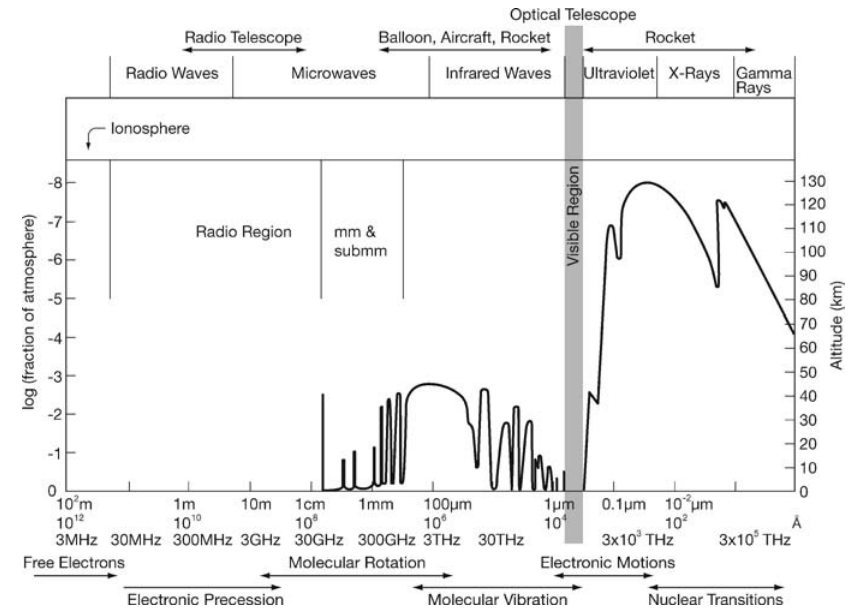
\includegraphics[width=0.6\textwidth]{images/radio_window.png}
 \caption[The radio window]{The radio window - Earth-based radio astronomy is bound to a range of wavelengths between $\lambda\approx 0.2mm$ and $\lambda\approx 20m$, by the molecular absorption bands of oxygen and water at
 shorter wavelengths and the ionosphere at longer wavelengths. The figure shows at what altitude the incoming electromagnetic radiation is attenuated by a factor of 0.5. Image taken from \textit{Tools of Radio Astronomy}~\cite{wilson2009tools}.}
 \label{fig_radio_window}
 \end{mdframed}
\end{figure}

In the early 1930s Karl Jansky's observation of radio electromagnetic radiation stemming from galactic sources far outside that of our home solar system sparked the interest in observing this region of 
the spectrum. Since those early days significant progress has been made towards increasing in the sensitivity and size of these radio telescopes. 

Next we will explore how a single element telescope works, before moving onto the topic of aperture synthesis with array-based telescopes.

\subsection{Radio antennae}
\subsubsection{Overview}
Maxwell's set of partial differential equations (1873) is one of the most elegant ways of explaining the relationship between electrical and magnetic fields, and how these can propagate at the speed of light 
though free space. In summary they state that a when current flows, a magnetic field is created in the surrounding space. When this magnetic field is varied a accompanying [perpendicular] electrical field is formed. This electrical field 
varies at the same frequency as the magnetic field, which in turn varies at the frequency at which the underlying current changes. Not only does this mean that antennae can generate electromagnetic fields and transmit signals (provided
sufficient input power), but in fact that any transmitting antenna can be used as a receiver and vice versa (given it is capable of dealing with high voltages and is efficient enough for the particular application domain). Radio telescopes 
take the form of receivers and, as with terrestrial radio transmission, the extraterrestrial electromagnetic radiation will induce measurable current in the antenna (much more so at shorter wavelengths 
because of the opaqueness of the ionosphere at longer wavelengths).

To simplify our discussion we'll only consider directional antennae (a simple parabolic reflector with an axial feed above the center of the parabola is 
one such choice). Here the parabolic reflector serve either to focus highly directional incoming energy to a single point, or inversely to 
focus the energy of the transmitter into a very narrow beam. Because the wavelengths of radio waves are the size of man-made objects the geometrical optics 
(where waves can be considered as rays) used in optical telescopes are of very limited use. It is much more preferable to describe these antennae in terms of 
physical optics.

Consider, for the moment, that the telescope is suspended in free space with no obstructions in its vicinity (including the ground or supports). If
we also (in blissful ignorance) discard the effects of the feed between this focus and measuring equipment, then the energy measured at the focus 
of the parabola should be the sum of contributions across the extent of the collected wavefront. However, instead of focusing all 
energy at one single point, as one would expect when using geometrical optics, an interference pattern is formed. Here
distinct beams can discernible (a close analogue to this is the interference pattern formed when light passes through a narrow slit).
If a cutting plane were to be placed horizontally at the focus of the parabola a single ``primary'' beam of maximum 
constructive interference will be noticed, along with several minor lobes to either side of that primary beam (the lobes right 
next to the primary beam are appropriately termed ``side'' lobes). Refer to Figure\ref{diffraction_pattern}. A highly directional antenna 
limits the maximum amplitude of these lobes considerably. It is important to note that an isotropic antenna will not have a single primary 
lobe, but may have several main lobes of equal amplitude. 

\begin{figure}[ht]
 \begin{mdframed}
  \centering
  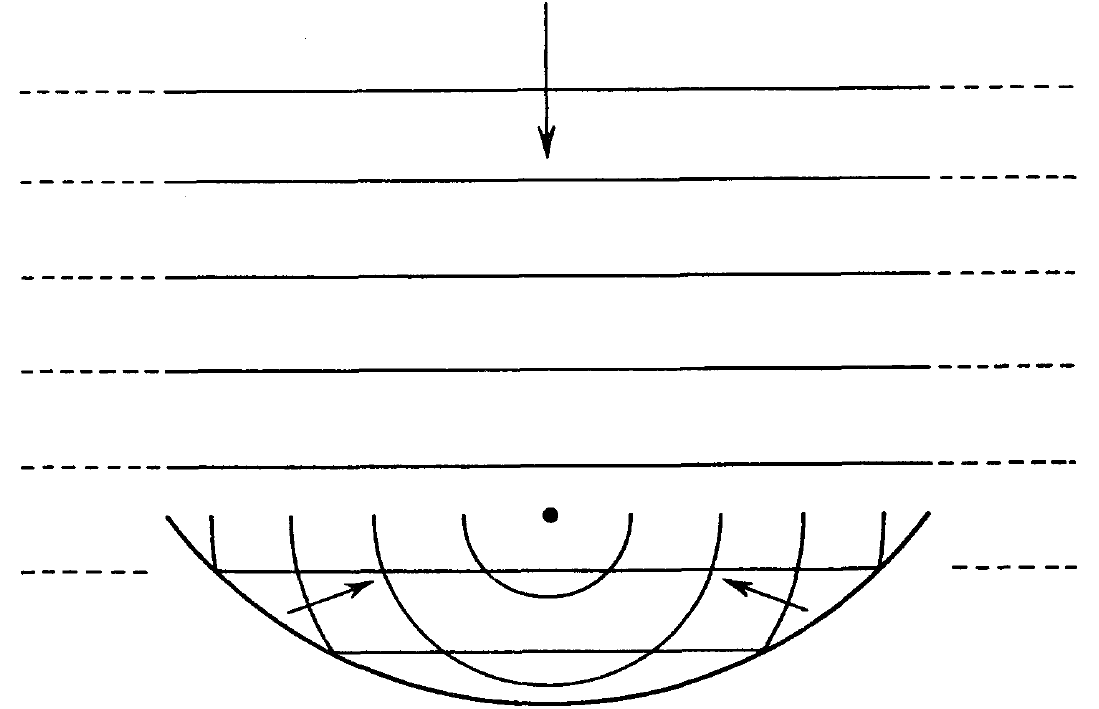
\includegraphics[width=0.4\textwidth]{images/diffraction_pattern.png}
  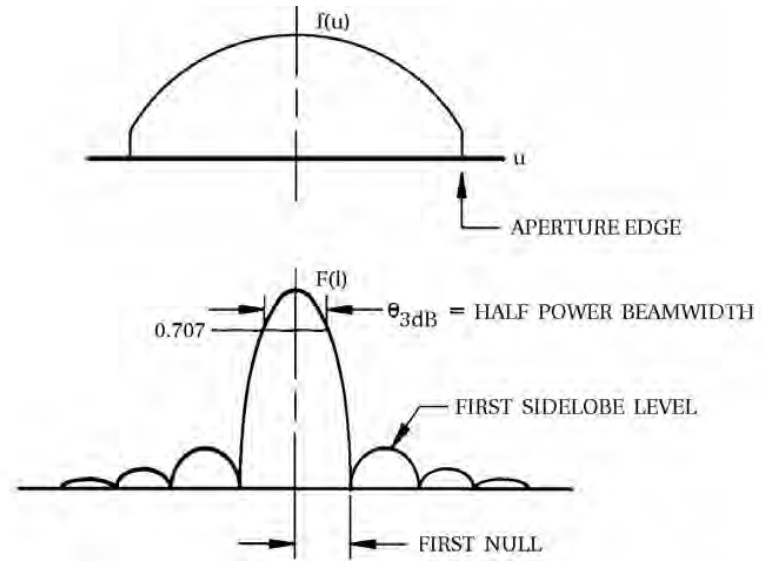
\includegraphics[width=0.5\textwidth]{images/radiation_pattern.png}
  \caption[Collection of electromagnetic wave energy and response]{Here the wave pattern of a parabolic aperture is 
  illustrated with a single cutting plane. The interference pattern created at the focus (illustrated on the right) is analogous to the interference pattern 
  of visible light when passing through a single narrow slit. Directional antennae form a discernible primary lobe, with several minor lobes of decreasing magnitudes to
  either side. The beam width of the primary lobe is [usually] defined as at the level where the electric intensity is halved (around $1/\sqrt{2}$ of the maximum response).
  At approximately $\frac{\lambda}{D}$ the ``first null'' appears ($D$ is the diameter of the aperture). This is the first point of complete destructive interference. When synthesizing
  an image  of a source which extends beyond the primary beam, one will notice a severe drop in the intensity of its edges. Images taken from \textit{Radiotelescopes} \cite{christiansenradiotelescopes} 
  and \textit{Synthesis Imaging II} \cite{taylor1999synthesis} (left and right respectively).}
  \label{diffraction_pattern}
 \end{mdframed}
\end{figure}

When placing the antenna back into a more realistic context: relatively close to the ground and taking the resistance of the feed connecting the antenna
to measuring equipment into account, this radiation pattern changes considerably (what is also referred to the ``absolute'' beam pattern).
As expected the ground (and any large nearby object will act as a reflector). Although the intensity of the reflection will vary depending
on how level the surrounding terrain is and its conductivity (dry or wet conditions) it cannot simply be ignored. Because the reflected wave may
be out of phase (depending on the height of the antenna and its declination) portions of the primary beam (in the vertical direction) 
may experience significant destructive interference.

The gain, $G$, of the antenna is defined as the ratio of radiation intensity collected in a given direction (as when emitted by a highly 
directional source), to the intensity that would have been obtained when receiving from an isotropic source. This definition includes feed losses
due to ordinary resistance and is obviously direction dependent. For our discussion on radio telescopes, however it is much more useful to think in terms of 
the effective area of the antenna. The effective area is defined in terms of the gain of the antenna:
\begin{equation*}
 A_e = \frac{G\lambda^2}{4\pi}
\end{equation*}
Assuming absolutely no losses occur in the measured electric density or any phase errors are introduced, this effective area will approach the geometric area of telescope in the direction
of maximum constructive interference. In practical application this is never achieved. The effective collecting area of the telescope is limited by a variety of
factors including, but not limited to, aperture surface deformation, blockage of the collecting area by support structs and the radiating properties of the feed.

It is worth pointing out that these radiating patterns are measured in the far field of the antenna (at distances at least $\frac{2D^2}{\lambda}$ from
the antenna where $D$ is the diameter of the aperture) to avoid any near-field reactive effects. The gain of an antenna must therefore be seen as a 
far-field concept.

In addition to the effective collecting area just defined, it must be pointed out that all antennae are only considered 
effective (depending on application constraints) for a limited spectrum of frequencies (or ``bandwidth''). This may be 
either a narrow or a wide band of frequencies. Note, however, that no real antenna system will cover a perfectly-rectangular band 
of frequencies. Effective lower and upper bands can be created by applying either analog or digital bandpass filters 
(a windowed sinc function is a commonly used filtering function). These filters have some finite \textit{rolloff} at both 
the lower and upper limits of the band and an inevitable trade-off between rolloff and rippling within the passband has to be made. 

Size is one of the factors governing effectiveness when it comes to bandwidth. Although there are no hard and fast rules about the size of antennae, 
some general rules of thumb are that antennae that are smaller than $0.5\lambda$ are considered electrically small and antennae more than 
about $100\lambda$ are considered electrically large, and are capable of attaining much higher gains in the case of directional antennae.

For astronomical purposes it is \textit{very important} to have an antenna much, much larger than $\lambda$. This is because some 
of the most important measurements of a celestial object includes the object's angular size, position (according to some celestial 
coordinate system) and the flux density over the frequency spectrum of the object. Although large objects may easily be resolved if
they are smaller than the primary beam, the resolution of finer details depend squarely on the angular resolution of the observing 
telescope:

\begin{equation*}
 \text{angular resolution} \propto \frac{\lambda}{D}
\end{equation*}
where:\\
  D \text{ is the aperture diameter}\\

Small telescopes will smear finer detail, and point sources right next to each other may not be discernible. The angular resolution is
an indication of the minimum distance at which two point sources can be separated and still be discernible. This sheds some light on astronomers'
never ending pursuit in building larger and larger antennae, as evident by the Arecibo observatory in Puerto Rico (Figure \ref{fig_arecibo}).

\begin{figure}[ht]
 \begin{mdframed}
 \centering
 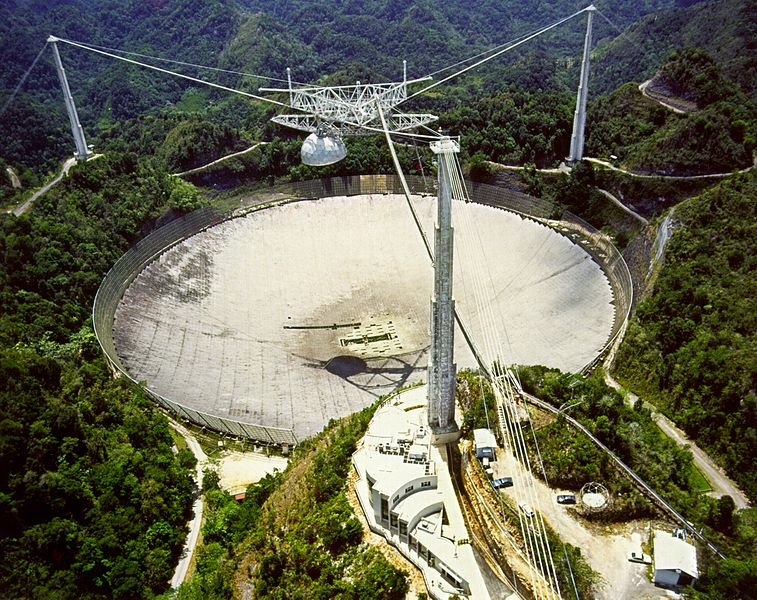
\includegraphics[width=0.7\textwidth]{images/arecibo.jpg}
 \caption[Arecibo Observatory]{At a wopping 305m diameter, the telescope at the Arecibo Observatory is amongst the largest single-apperature telescopes in the world. 
 Image courtesy of the National Oceanic and Atmospheric Administration (public domain).}
  \label{fig_arecibo}
 \end{mdframed}
\end{figure}

The variation of intensity over the emitting source and frequency are also of significant physical importance. Generally speaking, black-bodies (sources that near-perfectly absorb all incoming electromagnetic radiation)
will radiate this energy over a very wide band of the electromagnetic spectrum. Large bodies like planets and stars are generally considered to be of 
this type. The intensity distribution of black-body emission depends on both the equilibrium temperature of the body and the frequency of emission alluded 
to earlier. A black-body in equilibrium will [on average] have an emission intensity distribution that roughly follows the Plank 
distribution (Figure~\ref{fig_plank}). Here astronomers may choose to observe several bands that are widely spaced apart. In this \textit{continuum} 
observations much of the band may be averaged together without introducing error.

\begin{figure}[ht]
 \begin{mdframed}
 \centering
 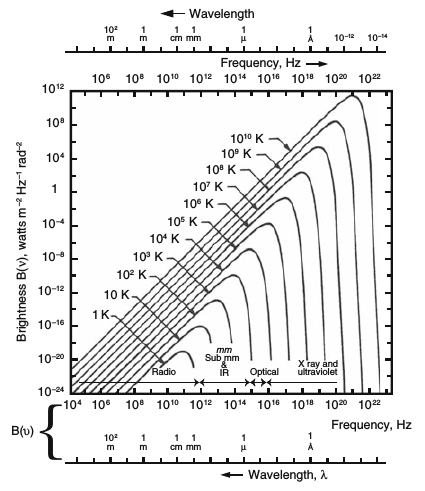
\includegraphics[width=0.4\textwidth]{images/plank_dist.png}
 \caption[Plank distribution]{The radiation intensity distribution for a black body in equilibrium. Taken from \textit{Tools of Radio Astronomy} \cite{wilson2009tools}}
  \label{fig_plank}
 \end{mdframed}
\end{figure}

This is by no means the only requirement from an astronomical perspective. Another may be to track the evolution of the universe. Astronomers are able
track certain very common elements, such as neutral hydrogen, by observing very narrow bands, discretized into many, densely spaced 
channels. These common elements absorb electromagnetic radiation at known frequencies ($\lambda = 21 cm$ for neutral hydrogen and
$\lambda \approx 18 cm$ for hydroxyl). These are appropriately called \textit{spectral line} observations and here data from different frequency channels
will be reduced independently.

\subsubsection{Measurement}
The energy available at the output terminals of a single aperture antenna will be roughly proportional to the electrical intensity per unit area per unit frequency on the 
collected planar wavefront. This is the electrical flux density, $S$ measured in units $Wm^{-2}Hz^{-1}$. It is useful to remind the reader that power is proportional to the square voltage and may 
practically be used interchangeably.

The single antenna telescope measures its power over a limited bandwidth and effective area $A_e$ as explained earlier. Assuming
no attenuation or delays are introduced by the atmosphere or equipment, and that the antenna measures two complementary polarizations, this 
means the total power measured by the telescope when pointed in the direction of a single point source is: 
\begin{equation*}
W = A_e.S.\Delta\nu
\end{equation*}

At this point it is necessary to introduce a rectangular coordinate system centered on the focus of the antenna, tilted such that w points 
in the direction of the maximum response, and u and v are the relative horizontal and vertical cutting planes respectively. u, v and w are 
measured in wavelengths (therefore measured in meters). The direction of a point on the sky (a unit sphere) is given by the 
direction cosines, measured according to the local frame. These cosines are denoted by l, m and n respectively (note that $l^2 + m^2 + n^2 = 1$). 
Both $l$ and $m$ may range between $\pm\pi \text{ radians}$.

Now let $\Omega$ be a \textit{small} solid angle subtended by a very small area. This solid angle is measured in square radians (steradians or ``sr''). A visualization 
of the measured flux density falling on an infinitesimal area of telescope is given in Figure~\ref{fig_measuring_source_brightness}. The flux density measured 
per steradian over the entire solid angle per unit frequency must then be 
  \begin{equation}
    p \approx \int_{\Omega}{A(l,m).I(l,m)\cos{\theta}d\Omega}
    \label{REF_EQN_SINGLE_ANTENNA}
  \end{equation}
where\\
  $p$ is traditionally measured in Janskies ($10^{-26}.W.m^{-2}.Hz^{-1}$)\\
  $I$ is the flux density measured per unit steridian: $I(l,m) := \frac{\Delta S(l,m)}{\Delta\Omega}$\\
\begin{figure}[ht]
\begin{mdframed}
 \centering
 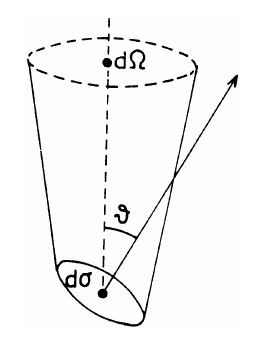
\includegraphics[width=0.2\textwidth]{images/measuring_source_brightness.png}
 \caption[Source brightness]{Flux density collected by a small area on the antenna. Image taken from \textit{Tools of radio astronomy}\cite{wilson2009tools}.}
 \label{fig_measuring_source_brightness}
\end{mdframed}
\end{figure}

In reality multiple sources will be contributing to this integral, each at a separate angle to the pointing center. The integral should therefore be taken over 
all contributing sources. It was assumed that these radiate independently of each other. Furthermore, the effects of the atmosphere, specifically frequency 
dependent delays and phase rotation, as well as tropospheric effects have been disregarded. The pointing accuracy and radiativity properties of the antenna including its internal 
temperature, polarization leakage, were also downplayed. Some of these effects can be corrected for through direct calibration and model-fitting techniques, 
but the exact details are beyond the scope of this introductory discussion. Typically calibration can be broken up into three areas:
\begin{itemize}
 \item \textbf{Direct calibration} involves data flagging. This type of calibration is normally used to mark broad portions of the data that is known to be invalid, due to for example
 technical malfunction. Modern radio astronomy software, for example the CASA reduction suite, have tools for performing this type of calibration.
 \item \textbf{Calibration through known calibrator sources and apriori information} 
 \item \textbf{Self-calibration processes} are iterative processes which typically involve model fitting algorithms and techniques.
\end{itemize}

For more details the reader is referred to Synthesis Imaging II \cite[Lectures 3, 5, 8 and 10]{taylor1999synthesis}. In the measurement section of the next chapter
we will refer to a general model which may be used to describe both atmospheric and antenna terms and can be used for self-calibration processes.

\subsection{Aperture synthesis with array telescopes}
\subsubsection{Overview}
As pointed out in the previous section the angular resolution is constrained to the diameter of the telescope. For longer 
wavelengths very big directional antennae are needed to achieve good angular resolution. Unfortunately 
there are material constraints, increased maintenance costs and a lack in steering capacity associated with large telescopes. 
Luckily it is not essential to build a filled aperture in order to create a reasonably efficient directional antenna. It is 
also possible to leave out large portions of the antenna aperture to create a directional antennae of significantly 
reduced weight (which is much cheaper to build). The obvious effect is a decrease in effective collecting area
and therefore decreased sensitivity.

Array telescopes can be thought of as a special case of these unfilled apertures. The very simplest way of creating such
a telescope will be to simply add the signals from all the receivers together before measurement, in order to form a 
basic ``total power'' telescope. This can be done only if the signals added together are reasonably \textit{coherent}. If they
are significantly out of phase the signals will experience significant destructive interference and the telescope will be
rendered useless. For the sake of discussion, however, it is assumed that the distances between antennae are fully taken 
into account: the wavefront collected at different locations will simultaneously arrive at the measurement equipment shortly 
thereafter, and the increased impedance associated with longer transmission lines is duly accounted for.

Using an array one is able to ``synthesize'' a single aperture telescope which encompasses the entire array. This
basic idea is known as \textit{aperture synthesis}. It does, however pose a serious conundrum: only some areas will be well covered, whereas
large areas may not be covered at all. As we see later on this produces smearing in the images produced and is a topic of much 
discussion by itself.

The resolving power obtained from such a synthesized aperture depends on the distance between the furthest separated 
telescopes, and can be expressed as:
\begin{equation*}
 \text{angular resolution} \propto \frac{\lambda}{B} \text{ if } D\ll B
\end{equation*}
where:\\
$D$ is the diameter of the largest aperture in the array and\\
$B$ is the length of the longest \textit{baseline} (the vector defined between the positions of pairs of antennae: 
either $\vec{b}_{pq}=P_p - P_q$ or $\vec{b}_{pq}=P_q - P_p$ depending on convention)

Since Martin Ryle and his associates made their pioneering observations using array telescopes there has been
a significant drive towards building arrays of ever-increasing size. In applications where angular resolution is
the one of the dominant factors it is even possible to connect up telescopes located on different continents, or even orbiting satellites.
This is appropriately called \textit{Very Long Baseline Interferometry}. A discussion on what is meant by an interferometer 
and why array telescopes are referred to as radio interferometers will follow very shortly (although it may be easy to guess given
the discussion on single antenna telescopes). In VLBI timing and data transport issues become major obstacles, and the data is usually 
physically shipped to a central location. Combination over the Internet (e-VLBI) has only recently become feasible. Avid readers may 
refer to the survey conducted by Middelberg et al. \cite{middelberg2008high} for a good introductory overview.

\subsubsection{Measurement}
It is also possible to think of arrays using a more physical approach. These telescopes measure what is commonly referred 
to as the \textit{spacial coherence} of a source. A simple analogy describing how array antennae work from a physical 
perspective would be to think of a point disturbance in a bowl of water. If the amplitude is measured by two calibrated 
sensors at the same location, the readings obtained should be exactly equal at any point in time. As the sensors are 
spaced further and further away from each other, but still equidistant to the source, one would expect the readings to still
be the same - since the waves propagate outward at the same speed and with the same amplitude. The degree to which
the two measurements correspond at any point in time will tell the observer how coherently the waves are propagating outward.

If this bowl of water analogy is scaled up to monstrous proportions, and the water is replaced with free space, it 
resembles an array telescope. Since the source is assumed to be sufficiently far away, each electromagnetic wave crest 
will be measured by two (or more) directional antennae at exactly the same time, provided those antennae point
towards the same sky position. Waves from directions $L.\cos{\alpha}=n$ will be in phase, but those from
directions $L.\cos{\alpha} = n + \frac{1}{2}$ will be out of phase ($n\in\mathbb{Z}$). Here $L$ is the length of the 
baseline $\vec{b}$ separating any two antennae. The delay between the arrival times is given 
by $\tau=\frac{\vec{b}\cdot\vec{s}}{c}$. Here $\vec{s}$ is the direction to the emitting source. See 
Figure~\ref{fig_interferometer}.

\begin{figure}[ht]
 \begin{mdframed}
 \centering
\psscalebox{1.0 1.0} % Change this value to rescale the drawing.
{
\begin{pspicture}(0,-5.5175757)(8.341955,5.5175757)
\definecolor{colour0}{rgb}{0.003921569,0.003921569,0.003921569}
\definecolor{colour1}{rgb}{0.0,0.047058824,1.0}
\rput{-226.70288}(-1.2319194,-5.399251){\psarc[linecolor=black, linewidth=0.02, fillstyle=solid,fillcolor=colour0, dimen=outer](0.5495573,-2.9655557){0.6944444}{7.8650684}{7.975039}}
\rput{-225.20427}(1.9264939,-5.7953396){\psarc[linecolor=black, linewidth=0.02, fillstyle=solid,fillcolor=colour0, dimen=outer](2.1695573,-2.4966667){1.31}{85.28396}{184.43335}}
\rput{-225.20427}(10.743828,-9.466027){\psarc[linecolor=black, linewidth=0.02, fillstyle=solid,fillcolor=colour0, dimen=outer](7.3422847,-2.4966667){1.31}{85.28396}{184.43335}}
\psline[linecolor=black, linewidth=0.02, arrowsize=0.05291666666666667cm 2.0,arrowlength=1.4,arrowinset=0.0]{->}(3.0904665,-0.43575758)(2.1177392,-3.3266666)
\psline[linecolor=black, linewidth=0.02, arrowsize=0.05291666666666667cm 2.0,arrowlength=1.4,arrowinset=0.0]{->}(8.245012,-0.4630303)(7.2722845,-3.3539393)
\psline[linecolor=black, linewidth=0.02, linestyle=dashed, dash=0.17638889cm 0.10583334cm](7.2722845,-3.3266666)(2.5904665,-1.9539394)
\rput{-19.51438}(1.2411542,0.5933079){\psarc[linecolor=black, linewidth=0.02, dimen=outer](2.3457046,-3.3121789){0.36926407}{33.895622}{125.547806}}
\psline[linecolor=black, linewidth=0.02, arrowsize=0.05291666666666667cm 2.0,arrowlength=1.4,arrowinset=0.0]{<->}(2.6995573,-3.2171428)(6.766224,-3.2266667)
\rput[bl](2.5449786,-2.984176){$\alpha$}
\psline[linecolor=red, linewidth=0.02, arrowsize=0.05291666666666667cm 2.0,arrowlength=1.4,arrowinset=0.0]{->}(7.270986,-3.312381)(7.213843,-0.4409524)
\rput[bl](7.070986,-0.32666665){$\vec{s_0}$}
\psline[linecolor=colour1, linewidth=0.02, arrowsize=0.05291666666666667cm 2.0,arrowlength=1.4,arrowinset=0.0]{->}(7.7836843,-2.2901587)(8.083684,-1.5473015)
\rput[bl](8.018605,-2.0726984){$\vec{s}$}
\psarc[linecolor=black, linewidth=0.02, dimen=outer](7.377335,-2.5481944){0.16736111}{0.0}{131.89452}
\rput[bl](7.299557,-2.7266667){$\theta$}
\psline[linecolor=black, linewidth=0.02, arrowsize=0.05291666666666667cm 2.0,arrowlength=1.4,arrowinset=0.0]{<->}(2.4450119,-1.9175757)(2.0086482,-3.2872727)
\rput[bl](1.4995573,-2.5842423){$\vec{b}\cdot\vec{s}$}
\rput[bl](4.0086484,-3.7236364){$||\vec{b}|| = L$}
\rput[bl](0.16622397,-2.3903031){$\tau=\frac{\vec{b}\cdot\vec{s}}{c}$}
\psline[linecolor=black, linewidth=0.02](2.1177392,-3.8084848)(2.0934968,-4.9721212)(4.493497,-4.9842424)
\psline[linecolor=black, linewidth=0.02](4.8934965,-4.9842424)(7.2934966,-4.9842424)(7.2934966,-3.7963636)
\psframe[linecolor=black, linewidth=0.02, fillstyle=solid,fillcolor=colour0, dimen=outer](4.917739,-4.7296968)(4.4813757,-5.2145452)
\rput[bl](3.9601634,-5.5175757){correlator}
\end{pspicture}
}
  \caption[Array-base observation]{In this simplified illustration of a two antenna array the incoming wavefront being measured is produced
  by a single source in the direction of $\vec{s}$, offset at an angle $\theta$ from the pointing center of the telescope $\vec{s_0}$.
  Here it is assumed that the pointing center is also the center of maximum response, where the delay between incoming signals
  is exactly zero. The \textit{correlator} measures the degree to which the signals measured at the two antennae correspond (
  both in phase and amplitude), therefore measuring the degree of spacial coherence of the incoming wavefront. For now we can assume
  the entire radio interferometer is on level ground, and importantly that the measured wavefronts are planar.}
  \label{fig_interferometer}
 \end{mdframed}
\end{figure}

These differences in phase depending on the angle of the incoming wavefront with respect to the pointing center will 
produce an interference phase pattern that is analogous to Young's double slit experiment, where an interference pattern 
is formed on a screen when light passes through two small slits (separated by a distance $L$) somewhere in front of the 
screen. Here the size of the slits are small in comparison to both $\lambda$ and $L$. The first null point occur at a distance 
proportional to $\frac{\lambda}{L}$. The only major difference between the two contexts is that the antennae should be
viewed as narrow slits.

This interference pattern is not ideal when resolving large structures. One way around this problem is to take an additional 
delayed measurement at $\tau_{delay}=\frac{\pi}{2}$ radians and combine this ``sine interference pattern'' to the original 
``cosine interference pattern''. In theory this improves the signal to noise ratio by a factor of roughly $\sqrt{2}$ and it will 
produce a response pattern that is sensitive over a wider range of angles. From this point forward whenever referring to the 
correlator we will be considering the \textit{complex} correlator. It is convenient to think of the measurements made by such a complex 
correlator in terms of the polar form of complex numbers. Recall Euler's famous identity:
\begin{equation*}
 e^{i\theta} = \cos{\theta} + i\sin{\theta}
\end{equation*}

As the reader may suspect the mathematical treatment of the measurements taken by these array telescopes are analogous
to that of a single aperture telescope, except that in the single antenna case the telescope measured the cosine modulated
flux density directly. Instead, here the signals are combined and measured by the external correlator. The mathematical 
discussion is very similar to that of a single antenna telescope, but will be that of a complex measurement, 
instead of only dealing with the real domain.

Up to this point it has been assumed that the signal will not vary over time, and that the measurement equipment is perfect; it 
does not delay or attenuate the collected signal (commonly referred to as the \textit{instrumental gain}). In reality however, 
this perfection is never attained. At a physical level, sources do vary slightly over time, although we expect their average 
intensity is centered around some mean. The instrumentation used for measuring will also contribute some variation that have to 
be corrected for on a regular basis (this will be described in more detail somewhat later on). The correlator should therefore 
measure the correlation over some short period of time in order to produce a reasonably accurate mean of the measured intensity. 
With this in mind it is important to make yet another assumption about the physical processes being measured: sources \textit{do not} 
vary significantly from their mean intensity on a day to day basis. It will soon become clear why this last assumption is essential.

The coordinate system defined for a single antenna telescope will have to be amended slightly to be relative to some fixed
location (it can be any) and the antennae in an array will be measured relative to this new coordinate frame. Assume
a single antenna is picked as reference point and all the other antennae positions are measured relative to this ``reference 
antenna''. 

This local [Euclidian] frame has the regular components X, Y, Z. If we use a right-handed system where X points in the direction 
of the $0^h$ hour hand, at a declination of $0^{\circ}$, Y lies on the same plane as X, but points to $18^h$ and Z points straight up 
towards the North Celestial Pole (NCP), then the baseline is given by the following relation, where $H_0$ and $\delta_0$ is the 
respective hour angle and declination of the phase reference center and $\lambda$ is the wavelength corresponding to the center 
frequency of the receiver. Refer to figure~\ref{fig_celestrial_coords} for a visual reference of the unit celestial sphere, and 
the equatorial and alt-azimuth coordinate systems. Here u, v, w are given by:
\begin{equation}
 \label{EQN_RIGHTHANDED_SYSTEM}
 \left[\begin{array}{c}
     u\\
     v \\
     w \\
    \end{array}\right] = \frac{1}{\lambda}
 \left[\begin{array}{c c c}
     \sin{H_0} 			& \cos{H_0}			& 0 \\
     -\sin{\delta_0}\cos{H_0} 	& \sin{\delta_0}\sin{H_0}	& \cos{\delta_0}\\
     \cos{\delta_0}\cos{H_0} 	& -\cos{\delta_0}\sin{H_0}	& \sin{\delta_0}\\
    \end{array}\right]   
 \left[\begin{array}{c}
     L_X \\
     L_Y \\
     L_Z \\
    \end{array}\right]
\end{equation}
The direction cosines towards a point on the celestial sphere is still given in relation to this relative u, v, w coordinate frame.
A similar left-handed convention can just as easily be defined ($\alpha_0$ is the right ascension of the pointing center):
\begin{equation}
 \left[\begin{array}{c}
     u\\
     v \\
     w \\
    \end{array}\right] = \frac{1}{\lambda}
 \left[\begin{array}{c c c}
     -\sin{\alpha_0} 			& \cos{\alpha_0}		& 0 \\
     -\sin{\delta_0}\cos{\alpha_0} 	& -\sin{\delta_0}\sin{\alpha_0}	& \cos{\delta_0}\\
     \cos{\delta_0}\cos{\alpha_0} 	& \cos{\delta_0}\sin{\alpha_0}	& \sin{\delta_0}\\
    \end{array}\right]   
 \left[\begin{array}{c}
     L_X \\
     L_Y \\
     L_Z \\
    \end{array}\right]
\end{equation}
\begin{figure}[h]
 \begin{mdframed}
 \centering
 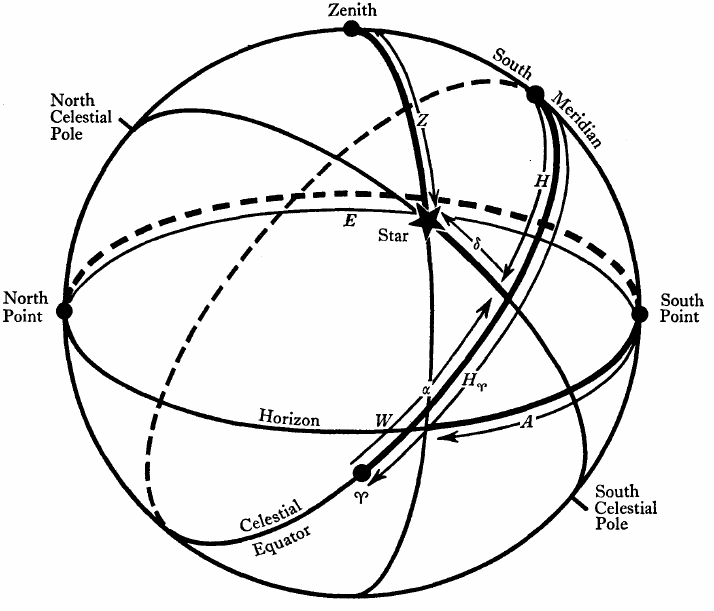
\includegraphics[width=0.75\textwidth]{images/equatorial_coords.png}
 \caption[Equatorial and alt-azimuth coordinate system]{The angular coordinates of a point in the sky can be measured in terms of declination ($\delta$) and either right-ascension ($\alpha$ or R.A.) or the hour angle ($H$) from the place
 where observations are taken (a celestial coordinate system). The first point of Aries (\Aries) is the position of the Sun at the March Equinox. The celestrial equator is simply Earth's equator projected onto the celestial sphere. There is normally a slow precession in the Earth's
 axis and this has to be corrected for, based on some reference point in time (an epoch). The last epoch at the time of writing was at noon January 1, 2000. See Radiotelescopes \cite[Appendix 4]{christiansenradiotelescopes} for more information.}
  \label{fig_celestrial_coords}
 \end{mdframed}
\end{figure}

Ignoring the effects of polarization, the directional antenna gain (the beam, as before) and any atmospheric effects
for a moment, the correlator will measure values proportional to (stemming directly from equation~\ref{REF_EQN_SINGLE_ANTENNA}):
\begin{equation*}
  \begin{split}
    p(u,v,w) &\approx \left<\int\int_{sources}{E_p(\vec{s})E_q^*(\vec{s'})e^{2\pi i(\vec{b}\cdot\vec{s})}e^{-2\pi i(\vec{b}\cdot\vec{s'})}d\Omega_pd\Omega_q}\right>\\
	     &\approx \left<\int\int_{sources}{E_p(\vec{s})E_q^*(\vec{s'})e^{2\pi i(\vec{b}\cdot(\vec{s}-\vec{s'}))}d\Omega_pd\Omega_q}\right>\\
  \end{split}
\end{equation*}

Here E is the flux density over a small area. The assumption that two sources at differing locations are not strongly correlated (in other words spatially coherent) is
essential in order to simplify this relationship between flux densities and correlator output. Still assuming both source 
direction vectors ($\vec{s}$ and $\vec{s'}$) are unit vectors pointing to positions on the unit celestial sphere (sky) this
assumption implies that $<S_p(\vec{s})S_q^*(\vec{s'})> \neq 0$ only when $\vec{s} = \vec{s'}$. Also note that, since complex fluxes
are being measured by the correlator, it is necessary to take the short time averages of the complex conjugate (denoted $^{*}$)
of one of the antennae in order to measure the total flux contributed by both components - otherwise the difference between
them will be measured! The expression now simplifies to:
\begin{equation*}
 p(u,v,w) \approx \int_{sources}{B(\vec{s})e^{2\pi i(\vec{b}\cdot(\vec{s}))}d\Omega}
\end{equation*}
where:\\
$B(\vec{s}) = <E_p(\vec{s})E_q^*(\vec{s})>$\\

Notice that the expression for p is relative and depends only on the direction of each contributing source. Of course this
is all relative to the pointing centre of the telescope. We may multiply through by a complex exponential to add the appropriate 
delay which ensures measurements are taken relative to the pointing center. It may help to think of this as measuring the
incoming [complex] flux from direction $\theta$ as shown in Figure~\ref{fig_interferometer}:
\begin{equation}
 \label{EQN_ONE_CORR_RIME}
 \begin{split}
 p(u,v,w) &\approx \int_{sources}{B(\vec{s})e^{2\pi i(\vec{b}\cdot(\vec{s}-\vec{s_0}))}d\Omega}\\
	  &\approx \int\int_{sources}{B(l,m,n)e^{2\pi i(u\Delta l+v\Delta m+w(\sqrt{1-l^2-m^2}-1))}\frac{dldm}{\sqrt{1-l^2-m^2}}}\\
 \end{split}
\end{equation}

By no means should this model be taken as a rigirous dirivation, but we will use it none the less (and slightly ammend it 
along the way). A more rigorous derivation is given by Romney in \cite{taylor1999synthesis}[ch. 4].

In reality the fact that the flux is averaged over a small band of frequencies and, additionally, over short periods of 
time will result in smeared measurements. It is important to emphasize that the baselines between pairs of antennae are 
\textit{always} measured in terms of wavelength (and by relation frequency) as evident from Equation~\ref{EQN_RIGHTHANDED_SYSTEM}.
If one were to integrate over such limited bandwidth the problem becomes apparent: the correlator response
is modulated by $\Delta\nu\sinc{\pi\Delta\nu\tau}$ (sinc is defined as $\sinc{x} = \frac{\sin{x}}{x}$). As apparent from
Figure~\ref{fig_interferometer} $\tau$ depends on the orientation of the baseline with respect to source, as well as the length of the 
baseline. The correlator response will be maximum only when the source vector is normal to the baseline. Therefore the 
correlator must compensate for this delay.

Up to this point we conveniently only discussed correlator output between single feed antennae.
Just as in the case of a single antenna telescope the response from such a correlator will only be sensitive to highly 
directional sources. The correlator may therefore additionally correlate all four combinations between the two orthogonal 
feeds of each antenna to form a 2x2 matrix of short time averages. Without any loss of generality the flux density 
average ($B$) in equation~\ref{EQN_ONE_CORR_RIME} can be replaced to include all four averages. The exponential term 
then becomes a scalar 2x2 matrix.

The four Stokes paramters are an easy way to describe the polarization of the measured electromagnetic field. These 
are non-physical quantities, but they give an easy way to express the degree to which the field is linearly or circularly polarized
(and anything inbetween). Each of the parameters Q, U and V are linearly independent and discribe a position on the 
Poincar\'e Sphere (figure \ref{fig_poincare}). I is the total measured intensity. The coordinates of Q, U and V are
those given by:
\begin{equation}
\begin{split}
Q &= I\cos{2\chi}\cos{2\psi}\\
U &= I\cos{2\chi}\sin{2\psi}\\
V &= I\sin{2\chi}\\
\end{split}
\end{equation}

\begin{figure}
\begin{mdframed}
\centering
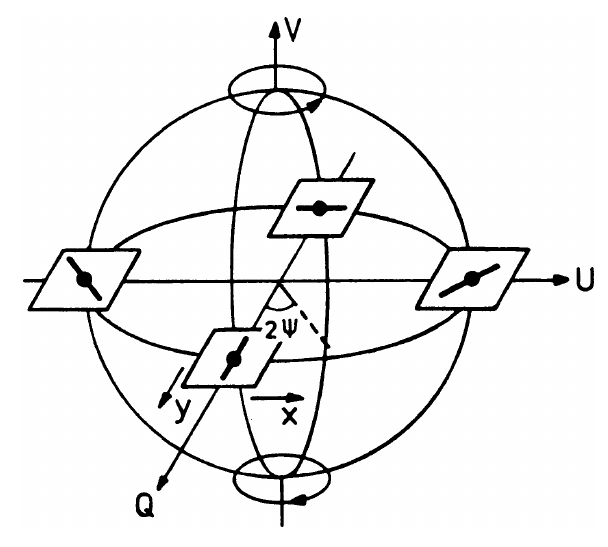
\includegraphics[width=0.45\textwidth]{images/poincare_sphere.png}
\caption[The Poincar\'e Sphere]{The Poincar\'e Sphere gives a visualization for the different polarizations an electromagnetic field. The angles $2\psi$ and
$2\chi$ are the angles in a polar coordinate system, with each point on the sphere corresponding to a unique polarization. At $2\chi=0$ (the equator) the polarizations
are either linear (Q) or orthogonal (U). The northern latitudes ($2\chi > 0$) contain right-handed circular polarization, while the southern hemisphere
contains the left-handed circular polarizations. $I$ is not linearly independent and describes the total flux of the electromagnetic wave: 
$I = E_1^2 + E_2^2$ \cite{wilson2009tools}}
\label{fig_poincare}
\end{mdframed}
\end{figure}

In instances where all of these components are available will the observer be able to compute the polarization of
the observed radiation. If the feeds of both antennae are orthogonal circular feeds the relation to
the the four Stokes parameters is given by
\begin{equation}
    \left[\begin{array}{c c}
     <e_{R_p}e_{R_q}^*> & <e_{R_p}e_{L_q}^*> \\
     <e_{L_p}e_{R_q}^*> & <e_{L_p}e_{L_q}^*> \\
    \end{array}\right] \approx 
    \left[\begin{array}{c c}
     I + V & Q + iU \\
     Q - iU & I - V \\
    \end{array}\right] = B
\end{equation}

For linear orthogonal feeds the relationship is slightly different \cite{2011A&A...527A.106S}:
\begin{equation}
    \left[\begin{array}{c c}
     <e_{X_p}e_{X_q}^*> & <e_{X_p}e_{Y_q}^*> \\
     <e_{Y_p}e_{X_q}^*> & <e_{Y_p}e_{Y_q}^*> \\
    \end{array}\right] \approx 
    \left[\begin{array}{c c}
     I + Q & U + iV \\
     U - iV & I - Q \\
    \end{array}\right] = B
\end{equation}

Equation~\ref{EQN_ONE_CORR_RIME} may thus be rewritten to take multiple polarizations, equipment gains and directional effects into account through a \textit{Jones} matrices 
formulation presented by Smirnov in a series of papers where he discusses their implications for telescope calibration \cite{2011A&A...527A.106S,2011A&A...527A.107S,2011A&A...527A.108S,2011A&A...531A.159S}:

\begin{equation}
\label{eqn_RIME}
\begin{split}
    V_{pq} &= G_p(t,\upsilon)\left(\int\int_{sources}D_p(l,m,t,\upsilon)BK_{pq}D_q(l,m,t,\upsilon)^H\frac{dldm}{\sqrt{1-l^2-m^2}}\right)G_q(t,\upsilon)^H\\
	  &\text{where }K = e^{2\pi i(u_{pq}l+v_{pq}m+w_{pq}(n-1))}
    \left[\begin{array}{c c}
     1 & 0 \\
     0 & 1 \\
    \end{array}\right]\\
	 &\text{and the G terms are the direction-independent effects,}\\
 	 &\text{while the D terms are dependent on the direction of the source in l,m space}\\
 	 &J^H:=\bar J^T \text{ indicates the Hermitian transpose (the transpose of the complex conjugate matrix of all the J indicies)}\\ 
\end{split}
\end{equation}

We shall henceforth refer to this relation as the \textit{Radio Interferometric Measurement Equation (RIME)}. 
The fundamental assumption here is that all effects on the measured intensities are linear and can therefore be 
written as two-dimensional matrices. Each antenna will have its own set of corrections. They 
include corrections for Faraday rotation, ionospheric effects, tropospheric effects, the primary beam (and any rotation during
observation) and pointing error due to weather (wind for instance). These corrections only account for amplitude scaling and 
phase shifts and can be combined in a layered approach by multiplying several of these Jones terms together (note that the terms 
may not necessarily commute, so the order of multiplication is important). We will come back to exactly how these terms are applied
when discussing on how the RIME can be inverted.

Up to this point the formulation was only made for two element arrays. However, the linearity of the system allows us
to simply add multiple of these short term averages together. When discussing signal processing aspects more formally
it will become clear why this may be done. In practice we can correlate the signal between all possible pairs of 
antennae and only reduce afterwards. This means that the data rates produced in correlation grows quadratically with 
number of antennae (ie. the number of possible baselines). This includes the auto-correlated baselines (correlation 
of each antenna with itself).
\begin{equation}
  \text{number of baselines } = \frac{n(n-1)}{2} + n
\end{equation}

Inquisitive readers may rightfully argue that even if many baselines are used to synthesize an aperture it will still be
very sparsely sampled, especially when considering very large arrays. In fact only a handful of small points will be 
sampled during a single integration period - hardly enough to represent a large continuous area! This means that 
the array telescope will be quite insensitive to very faint sources.

The solution to this problem lies in the beauty of the underpinning model we just developed: the flux measurements
are \textit{relative}. Recall also that the assumption that the intensity of the sources of electromagnetic radiation 
\textit{do not vary on a day-to-day basis}. This means an astronomer may fix one end of the baseline, and move the other
end. Some of the early radio telescope arrays did just this. Although many of the antennae were stationary a handful
of antennae were placed on tracks. These antennae would be moved to different positions to take multiple observations
of the sky.

Another, more promising, way of achieving this with much larger arrays is to use the rotation of the earth to rotate
the baselines radially with respect to the rotation axis of the planet. This may sound strange, but it 
follows naturally from the way the local coordinate frame was defined in Equation~\ref{EQN_RIGHTHANDED_SYSTEM}. If the
array tracks some point on the sky at some fixed declination over an extended period of time, the change in the hour
angle will rotate every baseline. This becomes clearer when recasting the equation from parametric to implicit form. 

Start by obtaining the individual expressions for u,v,w in equation~\ref{EQN_RIGHTHANDED_SYSTEM}. If the expressions
for u and v are manipulated into the familiar form of an ellipse it is easy to show (although tedious) that the following
relation holds:
\begin{equation*}
 u^2 + \left(\frac{v-(L_Z/\lambda)\cos{\delta_0}}{\sin{\delta_0}}\right)^2 = \frac{L_X^2 + L_Y^2}{\lambda^2}
\end{equation*}

This ellipse is shifted along the v axis by $\frac{L_Z\cos{\delta_0}}{\lambda}$. The major axis has a length of 
$\frac{2\sqrt{L_X^2 + L_Y^2}}{\lambda}$. It also follows that at low declinations the baselines 
of a pure east-to-west array will be nearly parallel to the pointing direction of the telsecope.
Not only will the foremost antenna shadow the antennae behind it, but there will be little coverage of the u, v
frame and a very weak response if the $\tau$ is not corrected for. One way of improving u,v coverage is to add baselines
that are sufficiently perpendicular to the rotation of the Earth (as is done in the VLA). These baselines are rotated into
the w-direction and present a serious problem in imaging. We will come back to this when discussing wide-field imaging.

To make this more concrete consider a fictitious observation with the Extended Very Large Array. The antenna 
positions for all 27 antennae, available baselines and projected tracks are shown in Figure~\ref{fig_evla_observation}. With
increasing frequency these tracks expand outward. This means that it is possible to effectively increase coverage
by observing multiple frequencies and averaging them together. However, this will cause some radial smearing when
images are synthesized.

\begin{figure}[h]
 \begin{mdframed}
 \centering
 \begin{subfigure}[b]{0.3\textwidth}
  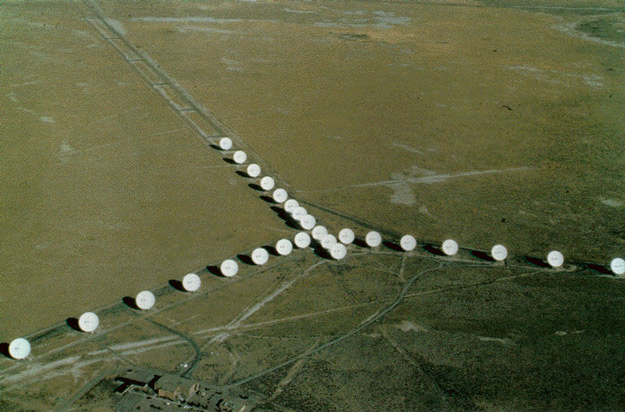
\includegraphics[width=\textwidth]{images/vla.jpg}
  \caption{}
 \end{subfigure}
 \begin{subfigure}[b]{0.3\textwidth}
  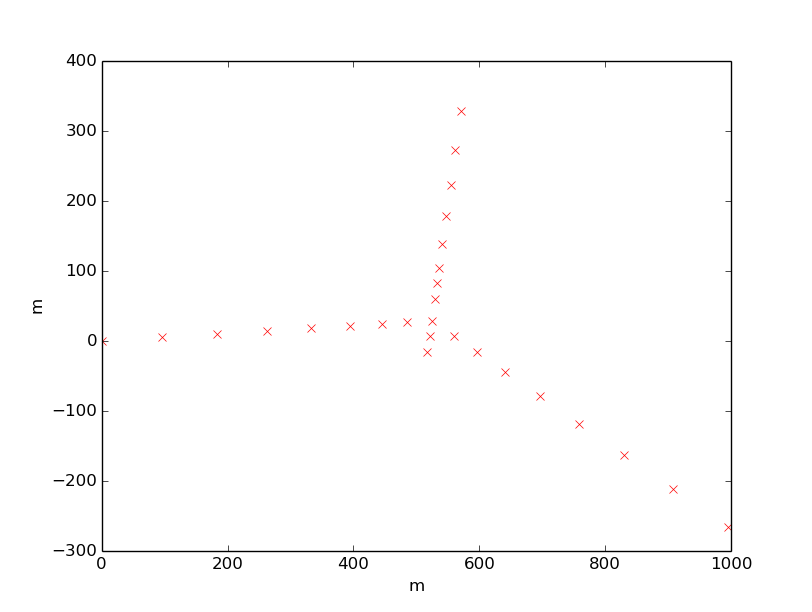
\includegraphics[width=\textwidth]{images/evla_observation/array_config.png}
  \caption{}
 \end{subfigure}
 \begin{subfigure}[b]{0.3\textwidth}
  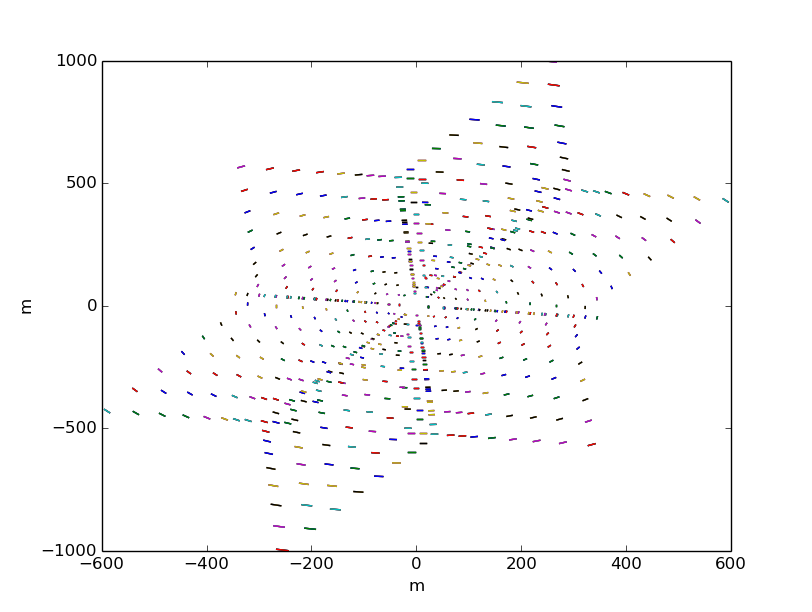
\includegraphics[width=\textwidth]{images/evla_observation/5min_snapshot_ncp.png}
  \caption{}
 \end{subfigure}
 \begin{subfigure}[b]{0.3\textwidth}
  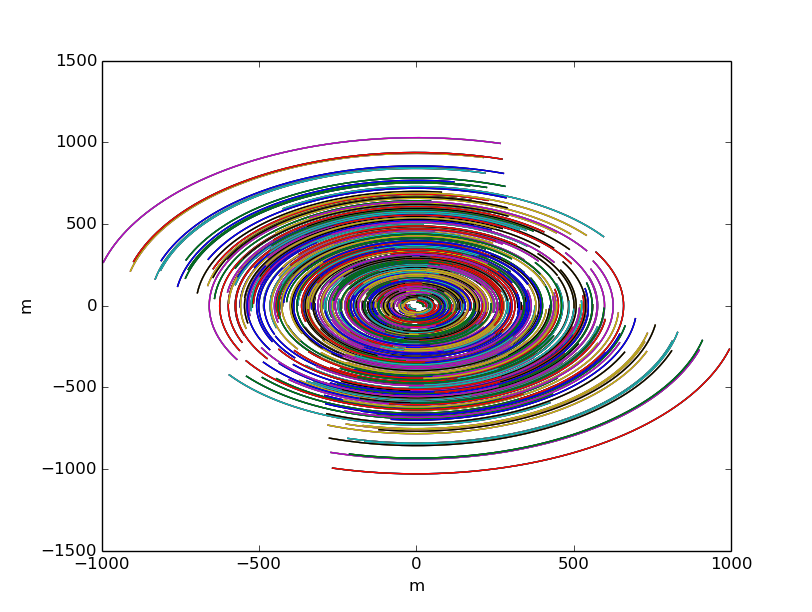
\includegraphics[width=\textwidth]{images/evla_observation/6hr_ncp.png}
  \caption{}
 \end{subfigure}
 \begin{subfigure}[b]{0.3\textwidth}
  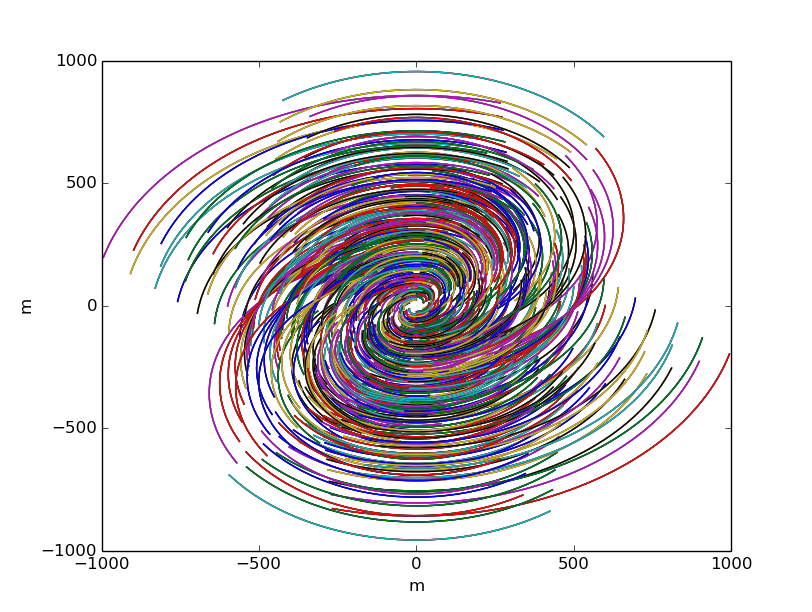
\includegraphics[width=\textwidth]{images/evla_observation/6hr_dec60.png}
  \caption{}
 \end{subfigure}
 \begin{subfigure}[b]{0.3\textwidth}
  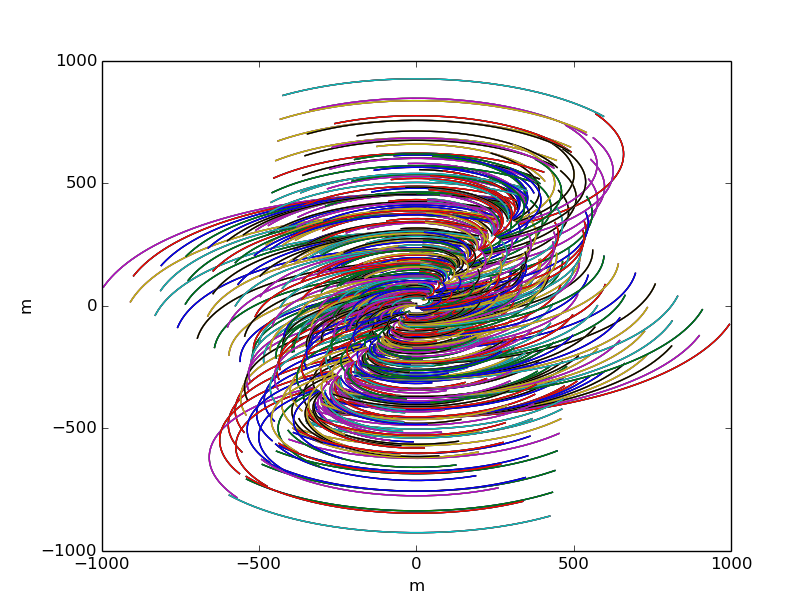
\includegraphics[width=\textwidth]{images/evla_observation/6hr_dec30.png}
  \caption{}
 \end{subfigure}
 \begin{subfigure}[b]{0.3\textwidth}
  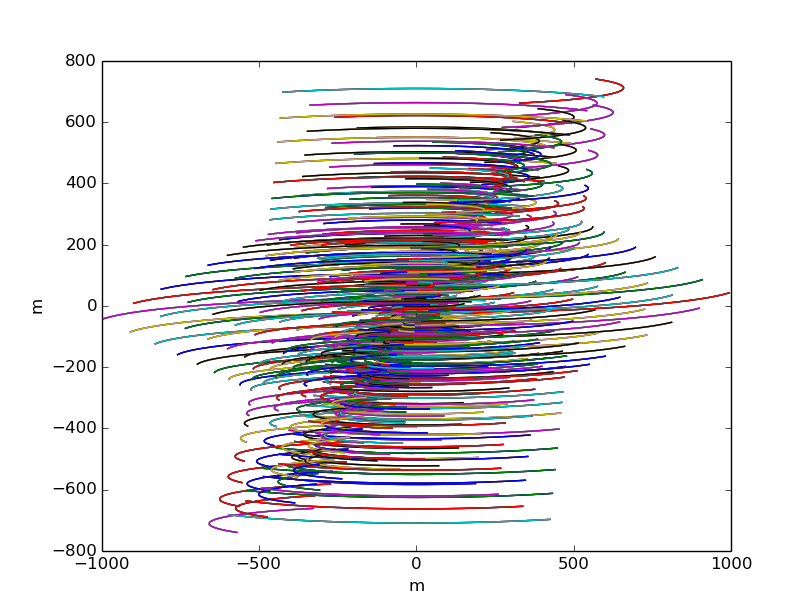
\includegraphics[width=\textwidth]{images/evla_observation/6hr_dec5.png}
  \caption{}
 \end{subfigure}
 \begin{subfigure}[b]{0.3\textwidth}
  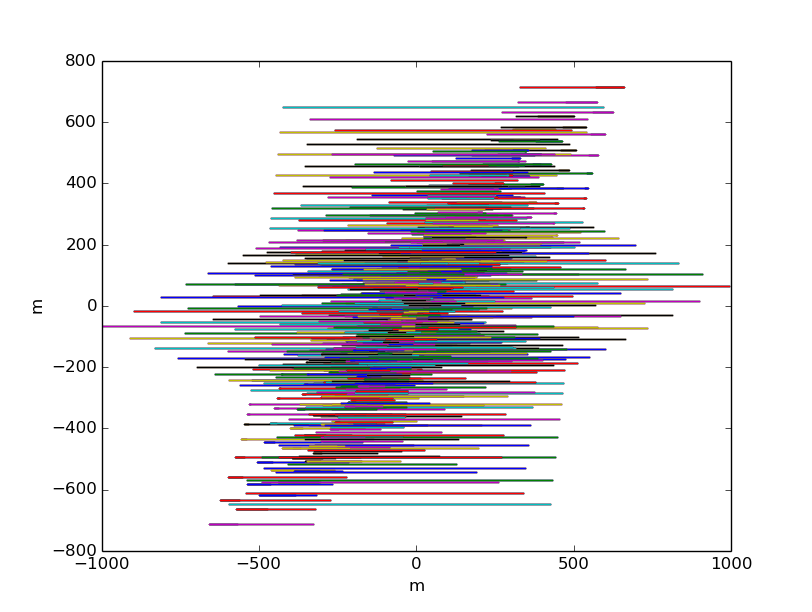
\includegraphics[width=\textwidth]{images/evla_observation/6hr_dec0.png}
  \caption{}
 \end{subfigure}
 \caption[u,v coverage]{Here the eliptical tracks from all baselines of the 27 antennae of the reconfigurable 
  Extended Very Large Array (National Radio Astronomy Observatory [New Mexico, US]) are shown at different declinations.
  In (a) a picture of the EVLA taken from \url{http://images.spaceref.com/news/2012/vla-625x412.jpg}. (b) shows the positions of the
  antennae when the array is in its compact ``D'' configuration. In (c) a 
  short (``snapshot'') 5min observation at NCP. In (d) a 6 hour observation at NCP. Figures (e)-(h) show 6 hour 
  observations for $\delta_0$ = $60^{\circ}$, $30^{\circ}$, $5^{\circ}$ and $0^{\circ}$ respectively.}
  \label{fig_evla_observation}
 \end{mdframed}
\end{figure}

%%%%%%%%%%%%%%%%%%%%%%%%%%%%%%%%%%%%%%%%%%%%%%%%%%%%%%%%%%%%%%%%%%%%%%%%%%%%%%%%%%%%%%%%%%% MORE ABOUT THE CORRELATOR ONCE WE DISCUSSED FOURIER THEORY

% It is worthwhile to note that the correlation, delay and phase compensations can also be done in the fourier domain, and in the case of delay compensation this approach makes fractional delay compensation feasible (see Taylor et al. \cite{taylor1999synthesis}). These correlators are effectively 
% known as \textit{FX} correlators. If these power spectra are of high time resolution it is possible to perform surveys focussed on transient detection. Modern arrays such as LOFAR, KAT-7 and MeerKAT (currently under construction) have the capability to perform these searches through
% special \textit{beamforming} modes which may be run concurrently with imaging modes. See Stappers et al. \cite{stappers2011observing} for details on pulsar observation with LOFAR. In this thesis, however, we will focus solely on the imaging pipeline which is discussed in the next section.
% 
% In the previous section the response, $r$, of a complex correlator was described. The \textit{visibility} is an unnormalized measure of the coherence of an electric field, and is very closely related to the correlator response to the planar wave fronts emitted
% by a source. The magnitude of this coherence has dimensions of flux density as described earlier. The Radio Interferometric Measurement Equation relates between these visibilities and the projection of the source onto the celestial sphere. This projection and measurement
% process is illustracted in figure~\ref{fig_uvw_lmn}. Without loss of generality when extended to the different polarization terms, the relation between the measured visibilities and the image can be defined as:
% \begin{equation}
%  \label{eqn_visibility}
%  \begin{split}
%   V(u,v,w) &:= \int_{\vec{s}}{A(\vec{s})I(\vec{s})\cos{\frac{2\pi\vec{b}\cdot(\vec{s}-\vec{s_0})}{\lambda}}d\Omega}\\
% 	   &= \int_{-\infty}^\infty{\int_{-\infty}^\infty{A(l,m)I(l,m)e^{-2\pi i[ul+vm+w(n-1)]} \frac{dldm}{\sqrt{1-l^2-m^2}}}}\\
% 	   &= \int_{-\infty}^\infty{\int_{-\infty}^\infty{A(l,m)I(l,m)e^{-2\pi i[ul+vm+w(\sqrt{1-l^2-m^2}-1)]} \frac{dldm}{\sqrt{1-l^2-m^2}}}}
%  \end{split}
% \end{equation}
% 
% \begin{figure}[h]
%  \begin{mdframed}
%  \centering
%  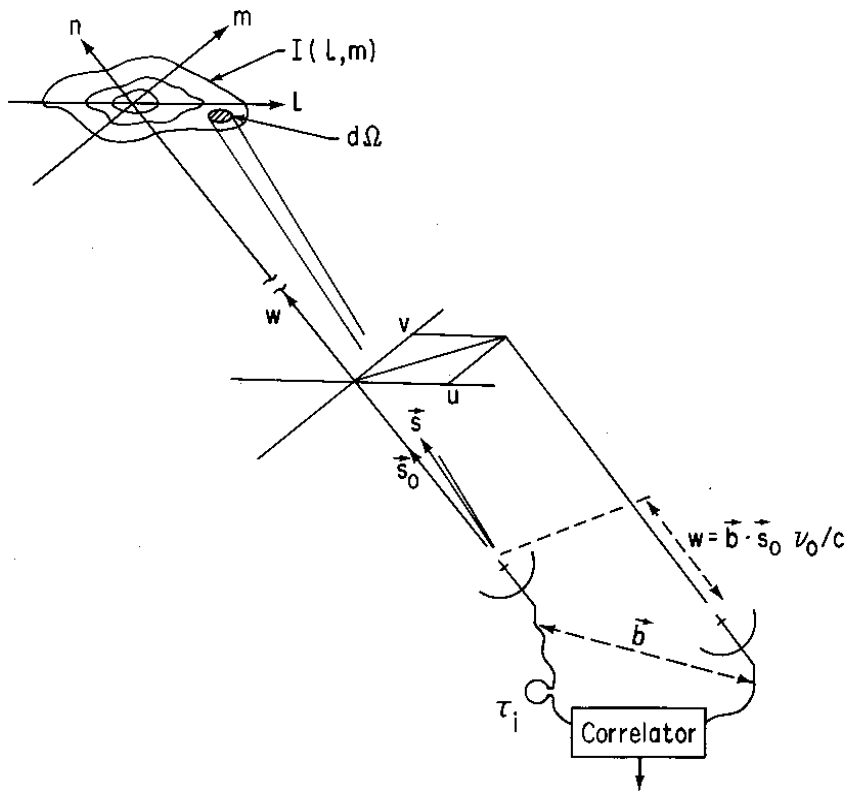
\includegraphics[width=0.5\textwidth]{images/lmn_uvw.png}
%  \caption[The relation between image space and visibilities]{The relation between the measured spatial coherence function and the source on the unit ``celestial'' sphere, emitting planar waves of radiation \cite{taylor1999synthesis}.}
%   \label{fig_uvw_lmn}
%  \end{mdframed}
% \end{figure}
% 
% When the field of view being observed is sufficiently small, $n$ is close to unity and the term $w(n-1) = 0$. Similarly, if the all the antenna are at equal height (\textit{co-planar}) $w=0$ and the term disappears as well. Under 
% these circumstances equation~\ref{eqn_visibility} is the two dimensional fourier transform of the image. In reality the image is not only affected by the effective area of the comprising elements in the interferometer, but is 
% subject to incomplete sampling, direction-independent antenna gains, as well as directional effects, such as ionospheric and tropospheric conditions. 
% 
% Each observation will typically extend over a prolonged period of time (over many hours for instance) and collect a large number of visibilities, typically over a large number of channels. As the earth rotates each baseline sweeps out
% eliptical paths in u,v space, sampling the coherence function at regular intervals. As the number of antennae in the array is increased the number of measured visibilities grow quadratically, since the number of possible baselines between 
% antennae is given as $\frac{n(n-1)}{2}+n$. Adding a small number of antennae to the array can therefore effectively improve the uv coverage. By adding more visibilities in fourier space the quality of the synthesized 
% image is improved, because the effects of the limited sampling can be more effectively removed from the produced image as is explained in the section on convolutional gridding.
% 
% The uniform and wide coverage of the entire u,v space (the size of which is determined by the required angular resolution), can normally be attained using only east-west baselines, except at very low declanations (less than about $30^o$) at the horizon. At low declanations baselines 
% with a component sufficiently parallel to the Earths axis (non East-West) are needed. Such a two dimensional array have baseline components which don't remain co-planar over long observations and require the l and m components being small enough to 
% ensure $(\sqrt{1 - l^2 - m^2} - 1)w \approx 0$. See figure~\ref{fig_VLBA_uv} for an illustration of the uv-coverage attained by the VLBA array. The spacing in such an East-West array is of high importance
% in ensuring the uniform sampling of the u,v space. Spacing the antennas uniformly for instance will result in many redundant coverages by the shorter baselines. Other designs include movable
% antennae provide greater flexibility and can cover more baselines. For two dimensional arrays reducing redundancy becomes even more challenging as eluded to in Synthesis Imaging II \cite[Lecture 2]{taylor1999synthesis}.
% 
% \begin{figure}[h]
%  \begin{mdframed}
%  \centering
%  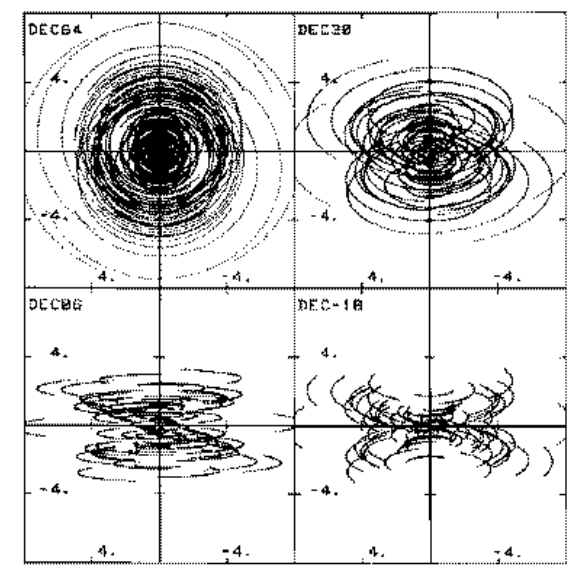
\includegraphics[width=0.5\textwidth]{images/eliptical_sampling.png}
%  \caption[VLBA uv-coverage]{The sampling patterns of the ten antennae of the VLBA at 4 different declanations. The best coverage is attained at greater declanations}
%   \label{fig_VLBA_uv}
%  \end{mdframed}
% \end{figure}
 
%%%%%%%%%%%%%%%%%%%%%%%%%%%%%%%%%%%%%%%%%%%%%%%%%%%%%%%%%%%%%%% CORRECTING THE RIME TERMS %%%%%%%%%%%%%%%%%%%%%%%%%%%%%%%%%%%%%%%%%%%%%%%%%%%%%%%%%%%%%%%%%%%%%%%% 
 
%  Correcting for known time-uniform directional effects can be achieved through either a facet-based polyhedron approach or through AW-projection. Using a image-space facet-based approach these directional
%  effects are locally-invariant and are corrected for over small portions of the final image, by multiplying with the appropriate inverse Jones matricies. In AW-projection these effects can be corrected for by convolving with
%  transposed Jones matricies, and this can be integrated to either the convolutional gridding (reverse Fast Fourier Transform) or degridding (forward Fast Fourier Transform) strategies which will be discussed 
%  in the next chapter \cite{2011A&A...527A.107S}. Both facet-based and AW-projection approaches will be discussed further in the chapter on non-coplanar wide-field imaging.
%  
%  Another approach is to subtract the directionally dependent effects directly from the observed visibilities, before correcting for the directional independent effects at the model
%  subtraction phase. Such an approach corrects these effects individually per model source and is equivalent to evaluating equation~\ref{eqn_RIME} for a set of discrete sources. These
%  analytical approaches are computationally prohibative, when compared to the convolution gridding approaches, coupled with either W-projection-based or faceting techniques, although 
%  it has the advantage of being much more accurate \cite{2011A&A...527A.107S}.
 
% \subsubsection{Self-calibration}
%  The lack of strong calibrators near observed areas, and the requirements placed on the properties of these calibrations, makes the process of calibrating the rapidly varying 
%  directional effects within the atmosphere a very hard problem. By allowing the individual element gains to be free parameters forms the basis of self-calibration. 
% 
%  Self-calibration imposes some restrictions: information about the absolute position, structure and intensity of an observed source is traded
%  for improved signal-to-noise ratios. It should be noted that these minimization approaches cannot completely replace the methods of source and polarization calibration mentioned earlier. 
%  The effect of these issues are normally incorporated as explicit Jones terms in the model, such as the one mentioned earlier. These effects are greatly reduced by adding additional 
%  antennae to the array. The self-calibration problem can be viewed as iteratively improving an initial model by correcting the effects of gain on sky brightness through algorithms such as the Maximum Entropy Method
%  and the CLEAN algorithm. The specification of the initial model does not necessarily have to be very accurate for CLEAN to converge at some point: it may simply 
%  consist of point sources for relatively simple images. Convergence is, however, not guarenteed.
% 
%  The H\"ogbom CLEAN algorithm locates (and keeps a list of) the brightest sources in an image in an iterative cycle, subtracting the Point Spread Function from each source until some 
%  thresholding condition is met. The remaining image is termed the residuals. After convolving the found point sources with elliptical function fitted over the Point Spread Function, 
%  the residuals are added to the convolved image, forming the final ''clean" image. Many other variations on the algorithm exist, bringing with them improvements in execution speed and 
%  stability.
% 
%  While CLEAN provides a procedural approach to deconvolution, the Maximum Entropy Method selects an image that fits the data to within a specified noise level, and is not procedural.
%  The method essentially limits the range of pixel values and focusses these ranges around bright objects. Though CLEAN is usually much faster on smaller simple images, it is prohibatively slow 
%  on large complex images. Under these conditions the Maximum Entropy Method is outright faster.
% 
%  Traditional self-calibration, however, assumes that the same ``apparent sky'' is sampled by all antennae, and solves only for the direction independent gain terms. They consider directional dependent terms as simple effects that 
%  do not vary in time and is identical per antenna. The addition of directional dependencies within the all-sky integral, primarily those caused by the ionosphere and modulation effects by the primary beam, violates this premis. In 
%  the NEWSTAR package the traditional self calibration process includes the following steps \cite{2011A&A...527A.107S}:
%  \begin{enumerate}
%   \item Gain minimization per antenna, and the minimization of the residual amplitudes and phases associated to each individual baseline (\textit{closure errors}) through a least squares approach.
%   \item Model subtraction to form a residual image.
%   \item Imaging, deconvolution and model updating using H\"ogbom CLEAN
%  \end{enumerate}
%  
%  In reality this simple least-squares gain-adjustment process cannot remove the effects due to polarized beam patterns, beam rotations and attenuation, as well as the aforementioned effects of the ionosphere and fast-varying tropospheric
%  effects. These directionally dependant effects are not simply a multiplication in u,v space, but should be thought of as a convolution. Because these effects vary with both direction and time, deconvolving them is an extremely tricky proposition: 
%  at every timestep since only a handful of points from these convolving functions are sampled! More recently several solutions to solve slow-varying Directional Dependent Effects using self-calibration have been proposed. These include pointing self-calibration,
%  peeling, the method of differential gains and other compressive sensing techniques (like the analytical solution descibed in \cite{hardy2013direct}). Peeling is a slightly modified version of traditional self-calibration and is widely tested. It involves iteratively removing the effects from the brightest sources, while 
%  differential gains simultaniously solves for the gain effects from bright and faint sources using a mix of Direct Fourier Transform and traditional Discrete Fourier Transform-based approaches \cite{2011A&A...527A.107S,2011A&A...527A.108S}.
 \section{Review of core digital signals processing techniques [need revision and simplification]}
Radio astronomy has its roots in Digital Signals Processing. Before diving into the details of how these telescopes work we refer the reader to the \textit{Scientist and Engineer's guide to Digital Signals Processing} by 
Steven Smith\footnote{Available freely at \url{http://www.dspguide.com/}}\cite{smith1997scientist} for a detailed, yet simple overview of the field. A (very) brief overview of some of the core terminology is given here.

A signal is simply a description of how one parameter depends on another. A typical example of this is how voltage varies over time. Since the focus in this thesis lie solely in digitized signals, it is necessary to carefully
define under what circumstances the underlying continuous analog signal can be reconstructed. The Shannon-Nyquest \textit{sampling theorem} forms the cornerstone of Digital Signals Processing. It simply states that the rate at
which samples are taken from a continuous signal has to be at least twice the highest frequency component of that signal. Such a signal is said to be critically sampled if it obeys this minimum requirement. If the requirement is
not satisfied the sampled signal is aliased (higher frequencies appear as low frequency com on gradebook and assignments tab yesterday on vula, so I thought I should contact you to know whether this is known to you. I don't know what happened but I had marks before. Thank you!ponents). This can be illustrated through figure~\ref{fig_invalid_sampling}. Aliasing is usually reduced by applying a filter that essentially
have low responses at frequencies outside a limited \text{passband} of frequencies. This filter is can be something as simple as a windowed sinc function for instance. Although a sharp cutoff frequency is ideal, it should be noted 
that in reality this is not achieved. Filter frequency responces usually decline over a non-infinitesimal section of the spectrum (this is known as \textit{rolloff}).

\begin{figure}[ht]
 \begin{mdframed}
 \centering
 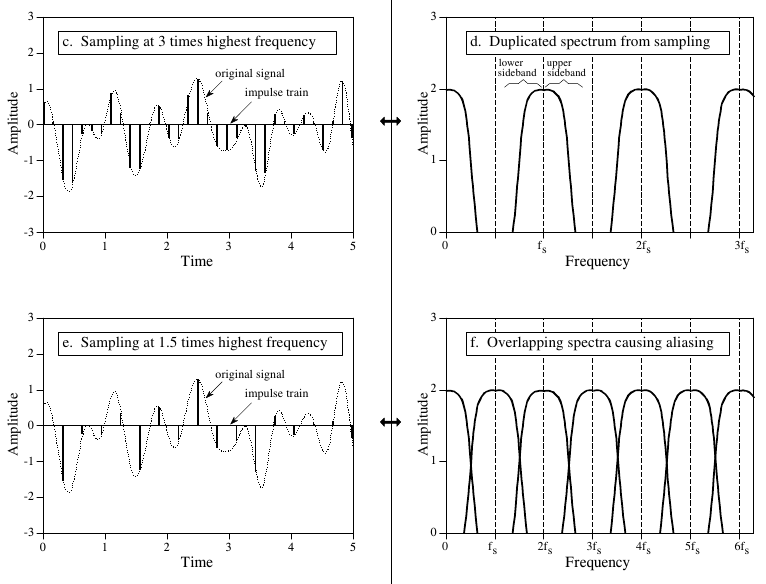
\includegraphics[width=0.8\textwidth]{images/improper_sampling.png}
 \caption[Aliasing]{The first signal is sampled at 3 times the highest composing frequency. Its frequency spectrum shows no overlap between sidebands. The second signal is subsampled and higher frequencies overlap lower frequencies
 in its frequency spectrum. This illustrates a key observation: discarding samples in one domain causes aliasing in the other \cite{smith1997scientist}.}
 \label{fig_invalid_sampling}
 \end{mdframed}
\end{figure}

The next observation is that the propogation of electromagnetic waves and their interactions can be considered as a linear system. This means the signals exhibit three properties: homogeneity, additivity and shift-invariance (the third 
is a non-compulsory property of linearity). We say that the following are true for such systems:

  \begin{flalign*}
    &\textbf{ if }x[n] \rightarrow \text{System} \rightarrow y[n] \textbf{ then } k x[n] \rightarrow \text{System} \rightarrow k y[n] \textit{ (homogeneity)}\\
    &\textbf{ if }x_1[n] \rightarrow \text{System} \rightarrow y_1[n]\textbf{ and }x_2[n] \rightarrow \text{System} \rightarrow y_2[n] \textbf{ then } x_1[n] + x_2[n] \rightarrow \text{System} \rightarrow y_1[n] + y_2[n] \textit{ (additivity)}\\
    &\textbf{ if }x[n] \rightarrow \text{System} \rightarrow y[n] \textbf{ then } x[n + s] \rightarrow \text{System} \rightarrow y[n + s] \textit{ (shift-invariance)}&
  \end{flalign*}

Much of the filtering and imaging techniques described in this thesis rely on the theory of fourier transforms. The fourier transform simply decomposes a continuous periodic signal into a series of sinusoidal terms. A detailed description 
can be found in Smith \cite[ch 8-12,31]{smith1997scientist}, but the general relations between converting between the time and frequency domains (and between the visibility and the intensity spaces as will be described later on) are as follows:
\begin{equation*}
  \begin{split}
    G(f) &= \int_{-\infty}^{\infty}g(x)e^{2\pi ifx}\\
    g(x) &= \int_{-\infty}^{\infty}G(f)e^{-2\pi ifx}
  \end{split}
\end{equation*}
Here capital letters indicate the Fourier space. We will be using this convention throughout this thesis. It is also possible to do this with discrete signals (indicated with square brackets as per convention). In that case the Cooley-Tukey Fast 
Fourier Transform algorithm and its inverse is employed to move between these domains. There are highly optimized libraries available for both C++ (FFTW) and CUDA (cuFFT), and these will be extensively used in our implementations.

For linear systems the following theorems are true (stated without proof):
\begin{equation*}
  \begin{split}
    g_1(x)*g_2(x) &:= \int_{-\infty}^{\infty}g_1(t)g_2(x-t)\textit{ (convolution)}\\
    g_1(x)\star g_2(x) &:= \int_{-\infty}^{\infty}g_1(t)g_2(t+x)\textit{ (cross-correlation)}\\
    &=g_1^*(-x)*g_2(x)\\
    \text{Addition Theorem:}\\
    \mathcal{F}(g_1(x)+g_2(x)) &= G_1(f)+G_2(f)\\
    \text{Convolution Theorem:}\\
    \mathcal{F}(g_1(x)*g_2(x)) &=G_1(f).G_2(f)\\
    \mathcal{F}(g_1(x).g_2(x)) &=G_1(f)*G_2(f)\\
    \text{Shift Theorem:}\\
    \mathcal{F}(g(x-\Delta))&=G(f)e^{-2\pi if\Delta}
  \end{split}
\end{equation*}

In general the convolution is known as filtering, the cross-correlation can be seen as ``time averaging between two signals'' and signal shifting essentially shifts the directional cosine (as seen in the next section) and electrically
stears the telescope. The two dimensional versions of convolution, cross-correlation, the fourier transform and its inverse are analoguous to their one dimensional counterparts. The two dimensional fourier transform first transforms
over one axis and then transforms the output on the second axis. 
 \section{The imaging and deconvolution pipeline [review and correct]}
 There are generally two techniques used to approximate the fourier transforms between the observed visibilities and the (dirty) image. Either a brute force Direct Fourier Transform is taken where each grid point is approximated through a brute-force
 evaluation over all the observed visibilities (M of them in total). This approach requires on the order of $O(N^2M) \approx O(N^4)$ sine and cosine evaluations (where N is the size of a single dimension of a square grid) for a large number of visibilities. A basic co-planar analytical 
 algorithm boils down to a summation of complex multiplications over the entire grid in the image space \cite[Lecture 7]{taylor1999synthesis}: 
 \begin{equation}
  (\forall \text{polarizations})(\forall l,m) I_{p}(l,m) = \frac{1}{M}\sum_{k=1}^{M}{V_p'(u_k,v_k)e^{2\pi i (u_kl,v_km)}}
 \end{equation}
 
 The second approach is to interpolate the data onto a regularly sampled grid with a two-dimensional convolution function, as is required when using the Fast Fourier Transform to approximate the transformations. A Fast Fourier Transform has a computational complexity of $O(N^2\log_2{N})$, while
 convolutional gridding typically requires $O(MC^2) \approx O(N^2C^2)$ operations (where C is the size of each dimension of a square filter) for large numbers of visibilities. If both the image size is small and the number of visibilities 
 are small the Direct Fourier Transform may be faster than the convolutional gridding approach. However, this will not generally be true for very large arrays such as the SKA or its predicessors that are currently under construction, 
 considering the sheer number of baselines involved, as well as the typical grid sizes involved.
 
 An abstract view of imaging, deconvolution and gain correction is shown in figure~\ref{fig_image_cycle}. Experiments performed by Varbanscu et al. \cite{varbanescu2008performance} show that convolutional 
 gridding accounts for nearly 35.4\% of the computation time, while the inverse process of degridding accounts for 48.74\% of a simple gridding and degridding cycle. In this chapter we will primarily focus on the convolutional gridding algorithm, optimal
 convolution functions and a brief overview of the inverse process is given. The next chapter discusses the problem of non-coplanar widefield imaging and the tradeoffs between the various solutions to the 
 problem. Therefore, the w term is, for the moment, not considered in this discussion.
 \begin{figure}[h]
 \begin{mdframed}
 \centering
 \begin{tikzpicture}[font=\tiny]
    \draw (0,0) rectangle (1.5,1) node at (0.75,0.5) {Antennae};
    \draw[->] (1.5,0.5) -- (2,0.5);
    \draw (2,0) rectangle (4,1) node at (3,0.5) {Interferometer};
    \draw[->] (4,0.5) -- (4.5,0.5);
    \draw (4.5,0) rectangle (6.5,1) node at (5.5,0.5) {Gain correction};
    \draw[->] (6.5,0.5) -- (7,0.5);
    \draw (7,0) rectangle (9,1) node at (8,0.5) {$V - V_{model}$};
    \draw[->] (8,1) -- (8,2);
    \draw (7,2) rectangle (9,3) node at (8,2.5) {Gridding};
    \draw[->] (8,3) -- (8,4) node[pos=.5, right]{Dirty $V_i^s$};
    \draw (7,4) rectangle (9,5) node at (8,4.5) {IFFT};
    \draw[->] (7,4.5) -- (6,4.5) node[pos=.5, above]{Dirty $I_i^s$};
    \draw (3,4.5) -- (4.5,4) -- (6,4.5) -- (4.5,5) -- cycle node at (4.5,4.5) {Converged};
    \draw[->] (3,4.5) -- (2,4.5);
    \draw (0,4) rectangle (2,5) node at (1,4.5) {Deconv. \& Update};
    \draw[->] (1,4) -- (1,3) node[pos=.5, right]{$I_{model}^s$};
    \draw (0,2) rectangle (2,3) node at (1,2.5) {FFT};
    \draw[->] (2,2.5) -- (3,2.5) node[pos=.5, above]{$V_{model}^s$};
    \draw (3,2) rectangle (6,3) node at (4.5,2.5) {Degridding};
    \draw[->] (5,2) -- (5,1) node[pos=.5, right]{$V_{model}$};
    \draw[->] (4.5,5) -- (4.5,6) node[pos=.5, right]{CLEAN $I_m^s$};
    \draw[style=thick] (4.4,6.1) -- (4.6,6.1);
    \draw[style=thick] (4.3,6.2) -- (4.7,6.2);
    \draw[->] (5,-1) -- (5,0) node[pos=.5, right]{A priori knowledge};
 \end{tikzpicture}
 \caption[Imaging pipeline]{The traditional imaging and deconvolution cycle. At the start of the cycle the data is flagged by the observer and known calibration and gain terms are provided.
 An Inverse Fast Fourier Transform is taken after the observed visibilities are uniformly gridded. This dirty sampled image is subsequently deconvolved and the model image updated as per 
 described in the previous section. After this an estimate of the deconvolved visibilities are obtained through an FFT and degridding process, depending on the approach taken. Normally several iterations 
 of this expensive self-calibration cycle is required to converge to a final image of reasonable quality. The directionally dependent effects can be reduced during either gridding 
 or degridding processes for an FFT-based approach. Analytical methods may vary significantly from this illustration.}
 \label{fig_image_cycle}
 \end{mdframed}
 \end{figure}
 
 Exploiting the computational efficiency of the Cooley-Tukey Fast Fourier Transform and its inverse to compute the forward and inverse Discrete Fourier Transforms requires, amongst other considerations, that
 the input is regularly sampled. This sampling is achieved through the process of convolutional gridding. In essense the algorithm can be broken down to four steps as illustrated in figure~\ref{fig_gridding}:
 \begin{enumerate}
  \item The individual complex visibilities are convolved with a highly oversampled function C(u,v). This process spreads them out accross a much wider area in u,v space.
  \item Afterwards the u,v space is regularly sampled.
  \item The image is computed through an Inverse Fast Fourier Transform
  \item A correcting function is applied to the sampled image.
 \end{enumerate}
 \begin{figure}[h]
  \begin{mdframed}
   \begin{tikzpicture}[font=\tiny]
    \filldraw[fill=red!20] (4.50,1.75) rectangle (5.25,2.5);
    \filldraw[fill=blue!20] (3.75,2.75) rectangle (4.50,3.50);
    \filldraw[fill=green!20] (5.50,4.75) rectangle (6.25,5.5);
    \draw[step=0.25,gray,thin] (3,1.5) grid (7,5.5);
    \draw[red] node at (0,0.25) {data at continuous coords (per baseline, per channel):};
    \draw node at (6.5,0.25) {\dots};
    \draw[step=1,black] (3,0) grid (6,0.5);
    \draw node at (3.5,0.25) {$u_0,v_0,\mathbb{C}$};
    \draw node at (4.5,0.25) {$u_1,v_1,\mathbb{C}$};
    \draw node at (5.5,0.25) {$u_2,v_2,\mathbb{C}$};
    \draw[->] (3.5,0.5) -- (5-0.125,2.25-0.125);
    \draw[->] (4.5,0.5) -- (4.25-0.125,3.25-0.125);
    \draw[->] (5.5,0.5) -- (6-0.125,5.25-0.125);
    \draw[->,gray] (3,1.5) -- (8,1.5) node[below,pos=0.5]{u};
    \draw[->,gray] (3,1.5) -- (3,6.5) node[left,pos=0.5]{v};
   \end{tikzpicture}
   \caption[Illustration of convolutional gridding]{Each observed visibility (per frequency channel and baseline) is centered at a precomputed coordinate in u,v space and is convolved with 
    some densely sampled function C and binned in a regularly spaced grid. This process essentially spreads each visibility out over a larger area in u,v space. The convolution function is typically sampled
    up to 100 times more regularly than the grid itself \cite{varbanescu2008performance,cornwell2007impact}. It should be clear that this is not the standard convolution as discussed earlier. The fact that the u,v coordinates may vary 
    significantly per baseline may result in two overlapping regions (this poses a problem when parallelizing the algorithm, as will be discussed later on). After all the observed visibilities have been gridded an 
    Inverse Fast Fourier Transform is performed and a correcting function is applied. Each polarization term is typically gridded and transformed to its own, independent, image.}
   \label{fig_gridding}
  \end{mdframed}
 \end{figure}
 Typically the u,v plane is only sparcely sampled as the earth rotates the baselines in u,v space as discussed earlier. This subsampling has the effect of multiplying the observed visibilities with a sampling function. It is also
 not uncommon to find that the u,v space is not uniformly sampled, as pointed out earlier, and that most of the samples are concentrated towards the center of the plane. It is convenient to weigh each sample with its neighbourhood density 
 (the number of visibilities in a neighborhood of grid cells) when sampling sources with both large- and small-scale structure. Natural sampling (typically a weight equal to 1) is used to detect faint sources. After fourier transform
 (by the convolution theorem) the transform of the sampling function is convolved with the image. In image space it is also generally referred to as the Point Spread Function or ``Dirty Beam''. It is possible to remove
 the effects of the Point Spread Function through deconvolution, but deconvolution generally requires a sufficient number of samples to obtain a satisfactory inverse \cite{taylor1999synthesis}.
 
 This sampled observed visibility plane is then convolved with a densely sampled convolution function. The primary goal of this convolution is to interpolate each visibility, but may also limit the aliasing energy outside the support 
 region of the convolving function, as well as limit the interpolation error introduced by using convolutional gridding, instead of the Direct Fourier Transform. Depending on the metrics used to define ``optimal gridding function'' these may vary from a simple truncated sinc or exponential function 
 \cite[Lecture 7]{taylor1999synthesis} to prolate spheriodal functions and approximations to these functions, such as the Keiser Bessel function \cite{jackson1991selection}. Sze Tan \cite{tan1986aperture} derives functions that out-perform prolate spheriodal functions
 on the basis of minimizing aliasing energy, as well as providing an opportunity to trade off the order of interpolation over the area for which the convolution error is small.
 
 It is possible to combine these operations into 
 \begin{equation*}
  I^s_{dirty} = ([I(l,m)*\mathcal{F}^{-1}\{PSF(u,v)\}]\cdot\mathcal{F}^{-1}\{C(u,v)\}) * \mathcal{F}^{-1}\{III(u,v)\}
 \end{equation*}
 \section{The problem of non-coplanar baselines and wide-field imaging [TODO: still have to be written]}
 {\color{red} TODO: WRITE THIS CHAPTER}
 Evaluating a direct 3D analytical solution over an image cube with n layers soon becomes intractable for large images, specifically in terms of sheer memory requirements for storing these layers. Over a three dimensional cube, M (the number of visibilities),
 will be reasonably sparcely sampled, and the number of complex multiplications needed per visibility is estimated to be $\frac{4\lambda B_{max}^3}{D^4}$ \cite{yashar2009tdp}. However, the approach remains embarisingly parallel and can
 be scalled over multiple multicore accelerators. A detailed comparison between the throughput achievable by using an analytical approach, compared to convolutional gridding approaches have not been for multicore accelerators \cite{hardy2013direct}.
 \section{Data formats [TODO:Still have to be written]}
 {\color{red} TODO: WRITE THIS CHAPTER}
 \section{Multicore architectures [TODO:Still have to be written]}
 {\color{red} TODO: WRITE THIS CHAPTER}
 \section{Review of previous literature [TODO:Still have to be written]}
 {\color{red} TODO: WRITE THIS CHAPTER}
\bibliography{bibfile}
\bibliographystyle{plain}
\end{document}          
